\documentclass[12pt,a4paper]{article}
% 12pt:     Tamaño de fuente
% a4papper: Tamaño de papel
% article:  Formato artículo, está dividido por secciones y subsecciones. Otros formatos: report, letter, book, etc.

\usepackage[spanish, es-tabla]{babel}
% Configura en español los nombres de figuras, tablas, etc.
\usepackage[utf8]{inputenc}                 % Permite el uso directo de tildes y otros.
\usepackage{amsmath,amssymb}
% Añade símbolos matemáticos para las ecuaciones.
\usepackage{parskip}
% Elimina la sangría
\usepackage{geometry}
% Permite modificar los márgenes de la página a gusto.
\usepackage{multicol}
% Ordena el cuerpo del documento en 2 o más columnas.
\usepackage{graphicx}
% Para poner imágenes.
\usepackage{enumitem}
% Para modificar los tags de los enumerate.
\usepackage{array}
% Para ordenar texto y ecuaciones.
\usepackage{url}
% Permite usar url que redirigen a la página web.
\usepackage{hyperref}
% Permite que se puedan clickear las urls, citas y referencias.

\spanishdecimal{.} % punto decimal
\geometry{margin=2cm} % margenes de la hoja
\renewcommand{\baselinestretch}{1.3} % tamaño de las filas de las tablas

\newcommand{\uveci}{\hat{\imath}} % vector unitario i
\newcommand{\uvecj}{\hat{\jmath}} % vector unitario j
\newcommand{\uveck}{\hat{k}} % vector unitario k

\begin{document}

\begin{center}
{\Large\textbf{INFORME N°2}}

{\LARGE\textbf{Suma vectorial y equilibrio de fuerzas}}

\rule{\textwidth}{0.5pt}

\begin{tabular}{ll}
    \textbf{Estudiantes:} & Catalina Lara Huenumán \\
                          & Daniel Lienan Gonzales \\
                          & Maximiliano Quezada Cornejo \\
                          & Samuel Saez Lozano \\[0.2cm]
    \textbf{Profesora:}   & Constanza Rivas \\
    \textbf{Ayudantes:}    & Lixin Lai \\
                           & Annelies Fullgraff \\[0.2cm]
    \textbf{Fecha de entrega:} & 23 de septiembre de 2026
\end{tabular}

\vspace{0.4cm}
\rule{\textwidth}{0.5pt}

\end{center}

\section{Procedimiento experimental}

\subsection{Parte 1 - Mediciones experimentales y suma gráfica de vectores} \label{Procedimiento-Parte-1}

Describan el procedimiento general utilizado para la realización de la medición de fuerzas y ángulos, la construcción de las configuraciones de equilibrio en la tabla de fuerzas y la representación gráfica de las fuerzas:

\begin{enumerate}[label=\alph*)]
\item Para el sistema de referencia se usó la escala angular impresa en la tabla de fuerzas. El ángulo $0^\circ$ se fijó en la dirección de la polea donde colgaban las masas, por lo que la fuerza $\vec{F}_1$ quedó siempre sobre el eje $+x$. Los demás ángulos se midieron en sentido antihorario a partir de ese eje;
\item Las masas se midieron con una balanza de resolución $0{,}01\,\mathrm{g}$. Los ángulos se leyeron directamente en la mesa, que está graduada cada $5^\circ$, así que se tomó como incertidumbre la mitad de esa división, $\delta\theta = 2{,}5^\circ$. Las fuerzas $\vec{F}_2$ y $\vec{F}_3$ se midieron con dinamómetros, considerando una incertidumbre de $\delta F = 0{,}01\,\mathrm{N}$;
\item La fuerza $\vec{F}_1$ no se midió directamente, sino que se calculó como el peso de las masas colgadas, $F_1 = mg$, usando $g = (9{,}81 \pm 0{,}01)\,\mathrm{m/s^2}$. Su incertidumbre se obtuvo por propagación de error a partir de $\Delta m$ y $\Delta g$;
\item Para armar cada configuración, primero se colgaron las masas en la polea del eje $+x$. Luego se engancharon los dos dinamómetros al centro de equilibrio mediante cuerdas y se ubicaron en los ángulos elegidos. Después se fueron ajustando las posiciones y tensiones hasta que el sistema quedara centrado en la tabla, momento en que se consideró que el sistema estaba en equilibrio y se anotaron las lecturas de los dinamómetros y los ángulos. En la Configuración 1 se usó una masa y los dinamómetros a $120^\circ$ y $240^\circ$; en la Configuración 2 se aumentó a 2 masas y se ubicaron a $150^\circ$ y $210^\circ$; y en la Configuración 3 se usaron tres masas, con los dinamómetros a $135^\circ$ y $300^\circ$;
\item Los vectores de cada configuración se graficaron en Python a partir de su módulo y ángulo, dibujándolos a escala desde el origen. Para la suma gráfica se usó el método del polígono, poniendo cada vector a continuación del anterior; si el sistema estuviera en equilibrio perfecto, el último vector terminaría justo en el origen, y la separación que queda corresponde a la resultante $\vec{R}_{\mathrm{exp}}$.
\end{enumerate}

\subsection{Parte 2 - Tratamiento analítico y propagación de error} \label{Procedimiento-Parte-2}

Para la suma analítica, cada fuerza se separó en sus componentes cartesianas usando su módulo y ángulo. Como tanto el módulo como el ángulo tienen incertidumbre, el error de cada componente se calculó por propagación, considerando ambos aportes y pasando $\delta\theta$ a radianes.
%Describan el desarrollo analítico utilizado para el cálculo de las componentes cartesianas de las fuerzas y sus respectivas incertidumbres absolutas.

Para las componentes $x$:
\begin{align*}
F_x &= F \cos\theta \\
\Delta F_x &= \sqrt{\left(\frac{\partial F_x}{\partial F}\delta F\right)^2 + \left(\frac{\partial F_x}{\partial \theta}\delta \theta_{\text{rad}}\right)^2} = \sqrt{\left(\cos\theta \, \Delta F\right)^2 + \left(-F\sin\theta \, \left(\Delta \theta \frac{\pi}{180^\circ}\right)\right)^2}
\end{align*}

Para las componentes $y$:
\begin{align*}
    F_y &= F \sin\theta \\
    \Delta F_y &= \sqrt{\left(\frac{\partial F_y}{\partial F}\delta F\right)^2 + \left(\frac{\partial F_y}{\partial \theta}\delta \theta_{\text{rad}}\right)^2} = \sqrt{\left(\sin\theta \, \Delta F\right)^2 + \left(F\cos\theta \, \left(\Delta \theta \frac{\pi}{180^\circ}\right)\right)^2}
\end{align*}

%Asimismo, detallen la forma analítica de calcular las componentes del vector resultante $\vec{R}_{\text{exp}}$ y sus incertidumbres $\Delta R_x$ y $\Delta R_y$:
Luego, las componentes de la resultante $\vec{R}_{\text{exp}}$ se obtuvieron sumando las componentes de las tres fuerzas, y sus incertidumbres sumando en cuadratura los errores de cada una:
\begin{align*}
R_x &= F_{1x} + F_{2x} + F_{3x}, \qquad \Delta R_x = \sqrt{\Delta F_{1x}^2 + \Delta F_{2x}^2 + \Delta F_{3x}^2} \\
R_y &= F_{1y} + F_{2y} + F_{3y}, \qquad \Delta R_y = \sqrt{\Delta F_{1y}^2 + \Delta F_{2y}^2 + \Delta F_{3y}^2}
\end{align*}

\subsection{Parte 3 - Comparación con la predicción teórica y análisis gráfico} \label{Procedimiento-Parte-3}

Para comparar con lo esperado teóricamente, se hizo en Python un gráfico de puntos con barras de error para cada configuración:

\begin{enumerate}[label=\alph*)]
\item En el eje horizontal se pusieron las componentes $R_x$ y $R_y$, y en el eje vertical su valor en newtons. La escala se ajustó en cada configuración para que se vieran bien los puntos y sus barras de error;
\item Cada punto se graficó con una barra de error vertical igual a su incertidumbre, $\pm\Delta R_x$ o $\pm\Delta R_y$, calculada como se explicó en la Sección \ref{Procedimiento-Parte-2};
\item Se trazó una línea horizontal en $y = 0\,\mathrm{N}$, que representa la condición de equilibrio $\sum \vec{F} = \vec{0}$, es decir, lo que se esperaría si las tres fuerzas se anularan completamente;
\item Para decidir si el resultado era compatible con el equilibrio se revisó si la barra de error de cada componente cruzaba la línea $y = 0\,\mathrm{N}$. Si la cruza, la diferencia con cero se explica por la incertidumbre de las mediciones; si no, indica una desviación probablemente causada por errores sistemáticos, como el roce en la polea o error en alguna medición.
\end{enumerate}

\newpage
\section{Configuración de Equilibrio 1}

En la primera configuración se utilizó una única masa suspendida, $m = (50{,}81 \pm 0{,}01)\,\mathrm{g}$, colgada de un hilo que pasa por una polea ubicada en el borde de la mesa de fuerzas sobre la dirección del eje $+x$. El peso de la masa, constituye la fuerza $\vec{F}_1$ ($\theta_1 = 0^\circ$). Las fuerzas $\vec{F}_2$ y $\vec{F}_3$ se aplicaron mediante dos dinamómetros fijados a $120^\circ$ y $240^\circ$ respecto al eje $+x$ (medidos en sentido antihorario), de modo que las tres fuerzas quedaran separadas simétricamente por $120^\circ$. La incertidumbre angular de la mesa se estimó en $\delta\theta = 2{,}50^\circ$ y la de los dinamómetros en $\delta F = 0{,}01\,\mathrm{N}$.

\begin{table}[h!]
\centering
\begin{tabular}{|c|c|c|}
\hline
\textbf{Fuerza} & \textbf{Módulo ($F \pm \delta F$)} & \textbf{Ángulo ($\theta \pm \delta \theta$)} \\ \hline
$F_1$ & $(0{,}498 \pm 0{,}001)\,\mathrm{N}$ & $(0{,}0 \pm 2{,}50)^\circ$ \\ \hline
$F_2$ & $(0{,}420 \pm 0{,}01)\,\mathrm{N}$ & $(120{,}0 \pm 2{,}50)^\circ$ \\ \hline
$F_3$ & $(0{,}470 \pm 0{,}01)\,\mathrm{N}$ & $(240{,}0 \pm 2{,}50)^\circ$ \\ \hline
\end{tabular}
\caption{Medición directa e indirecta de módulos y ángulos para la Configuración 1.}
\label{tab:config1-mediciones}
\end{table}

Los datos recolectados de esta configuración fueron registrados en la Tabla \ref{tab:config1-mediciones}. La representación gráfica de los vectores de esta configuración se puede ver en la Fig. \ref{fig:config1-vectores}.

\begin{figure}[h!]
    \centering
    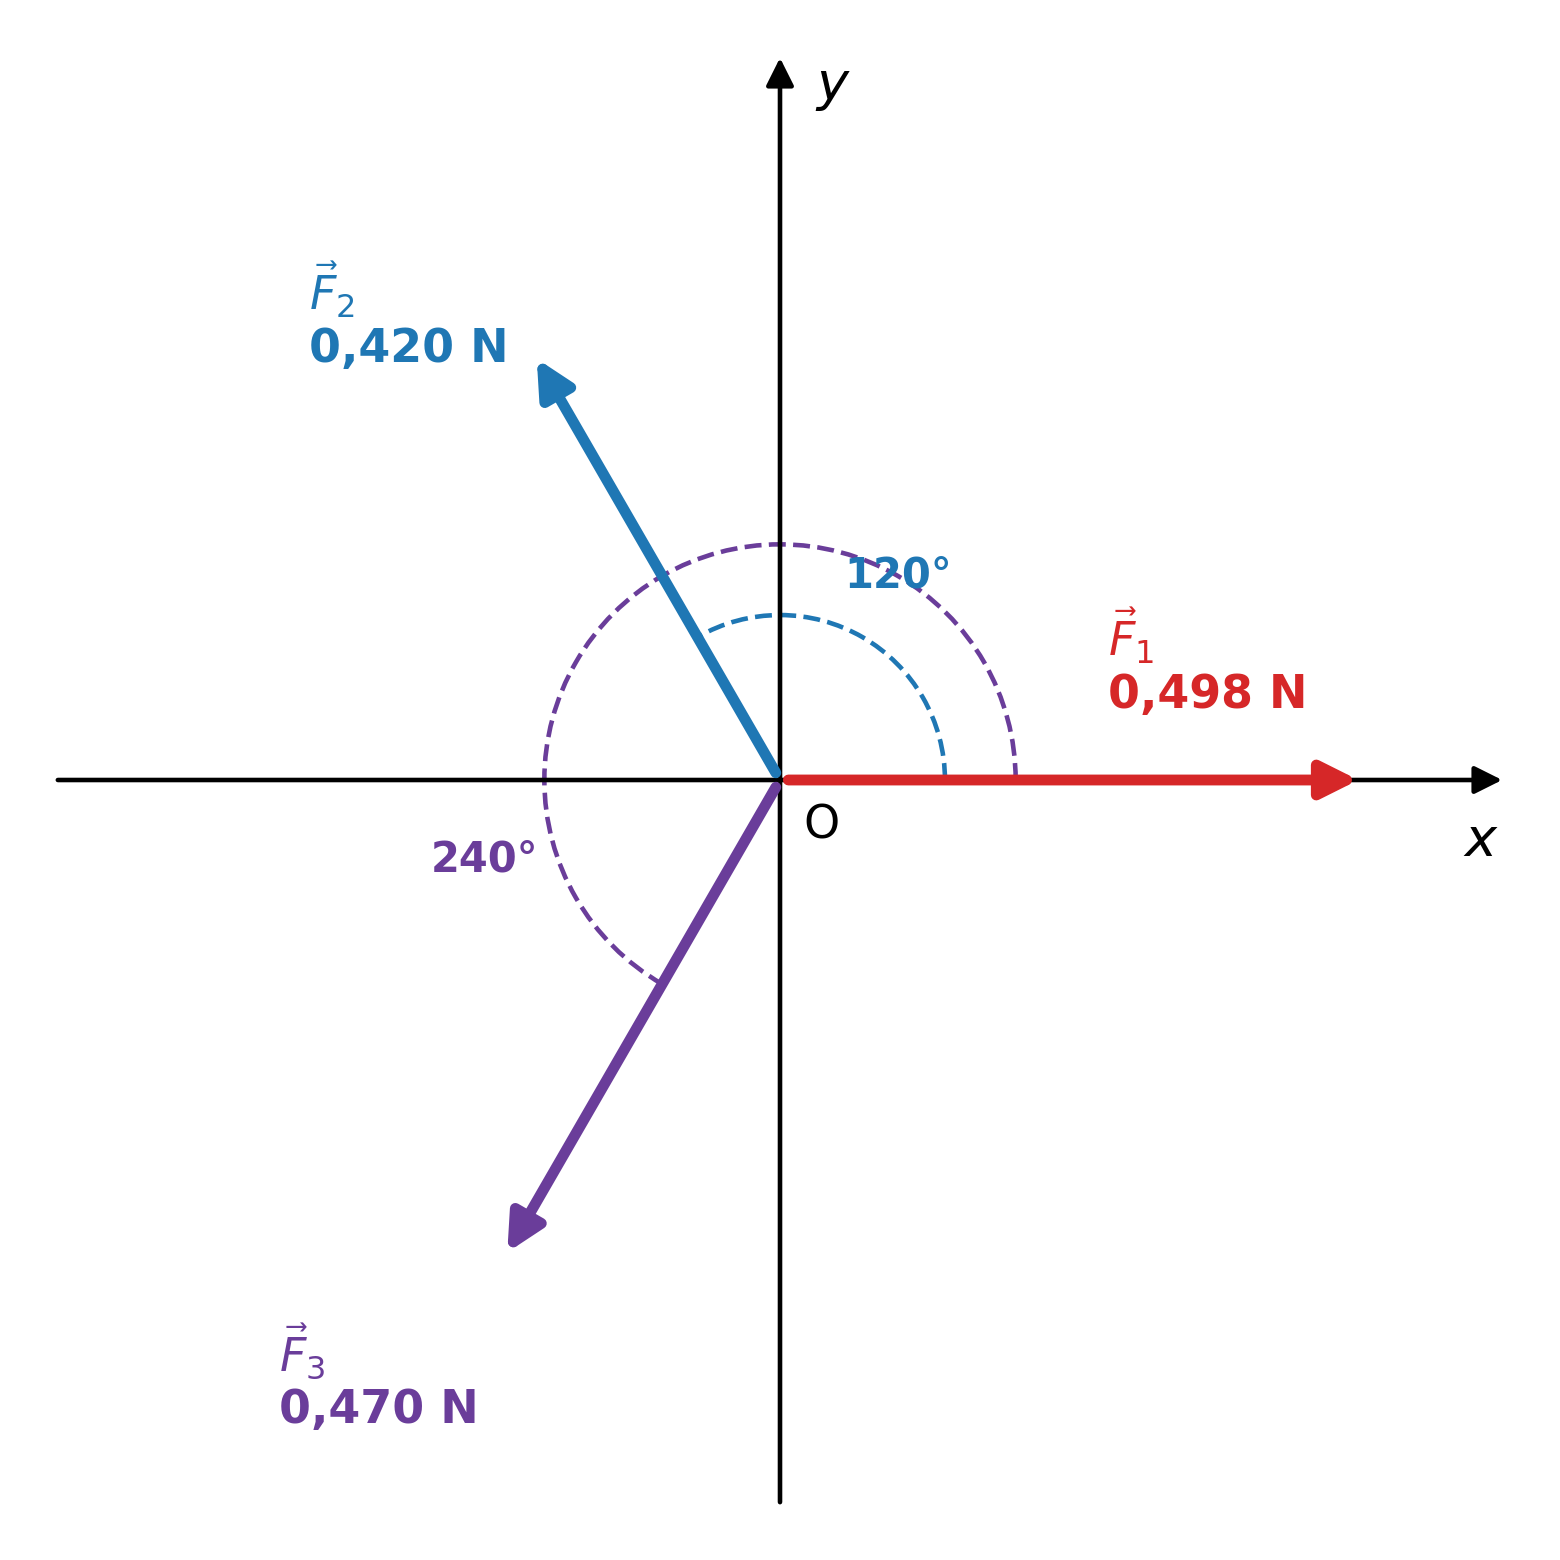
\includegraphics[width=0.4\textwidth]{config1-vectoress.png}
    \caption{Representación en el sistema de referencia de los vectores $\vec{F}_1$, $\vec{F}_2$ y $\vec{F}_3$ (Configuración 1).}
    \label{fig:config1-vectores}
\end{figure}

El módulo de $\vec{F}_1$ corresponde al peso de la masa, calculado como $F_1 = mg$. Para obtener $\delta F_1$, se realizó propagación de error.
\begin{equation*}
F_1 = mg = (0{,}05081\,\mathrm{kg})(9{,}81\,\mathrm{m/s^2}) = 0{,}498\,\mathrm{N} \dots
\end{equation*}
\begin{equation*}
\delta F_1 = \sqrt{\left(\frac{\partial F}{\partial m} \Delta m \right)^2 + \left(\frac{\partial F}{\partial g} \Delta g \right)^2} = \sqrt{(9{,}81 \times 0{,}00001)^2 + (0{,}05081 \times 0{,}01)^2}\;\mathrm{N} \approx 0{,}001\,\mathrm{N} \dots
\end{equation*}

\subsection{Suma gráfica}

La suma gráfica de los vectores se puede ver en la Fig. \ref{fig:config1-poligono}.

\begin{figure}[h!]
    \centering
    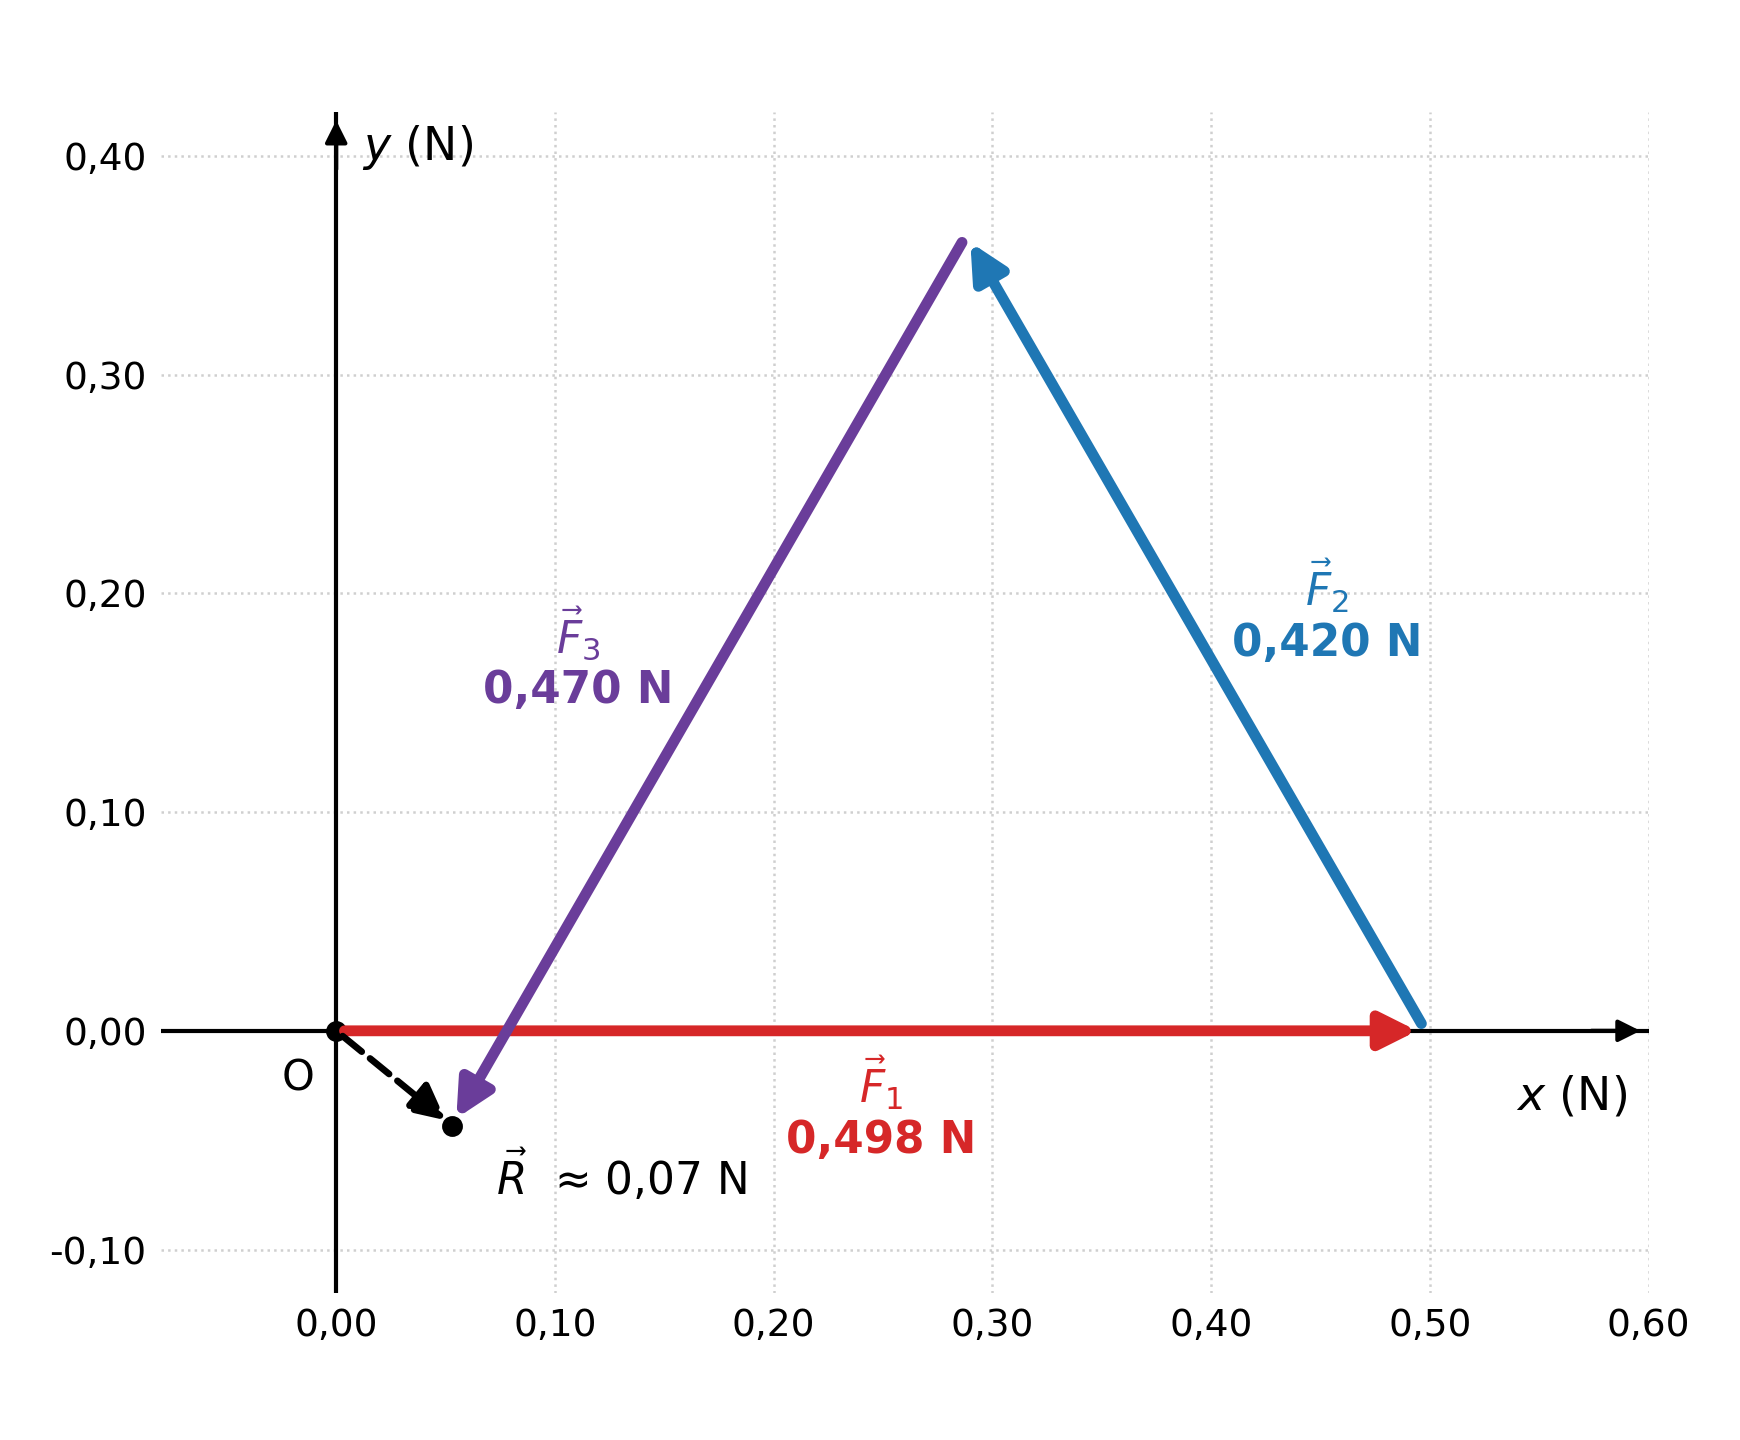
\includegraphics[width=0.4\textwidth]{config1-poligono.png}
    \caption{Suma gráfica mediante el método del polígono para la Configuración 1.}
    \label{fig:config1-poligono}
\end{figure}

Al trazar los vectores a escala uno a continuación del otro, el polígono no se cierra de forma exacta: entre el extremo de $\vec{F}_3$ y el origen de $\vec{F}_1$ queda una pequeña abertura, del orden de $0{,}07\,\mathrm{N}$ en la escala utilizada (aproximadamente un $14\,\%$ del módulo de $\vec{F}_1$). Esta discrepancia es coherente con que, para tres fuerzas separadas por $120^\circ$, el cierre exacto requiere módulos iguales, mientras que experimentalmente se obtuvo $F_1 > F_3 > F_2$.
%Comenten cualitativamente si el polígono se cierra correctamente o si existe alguna discrepancia gráfica visible.

\subsection{Suma analítica}

Los vectores de la Configuración 1 separados en sus componentes están registrados en la Tabla \ref{tab:config1-componentes}.

\begin{table}[h!]
\centering
\begin{tabular}{|c|c|c|}
\hline
\textbf{Fuerza} & $F_x \pm \Delta F_x\,\mathrm{(N)}$ & $F_y \pm \Delta F_y\,\mathrm{(N)}$ \\ \hline
$F_1$ & $0{,}498 \pm 0{,}001$ & $0{,}00 \pm 0{,}02$ \\ \hline
$F_2$ & $-0{,}210 \pm 0{,}016$ & $0{,}364 \pm 0{,}009$ \\ \hline
$F_3$ & $-0{,}235 \pm 0{,}018$ & $-0{,}407 \pm 0{,}010$ \\ \hline
\end{tabular}
\caption{Componentes cartesianas e incertidumbres absolutas para la Configuración 1.}
\label{tab:config1-componentes}
\end{table}

Sumando estas componentes, el vector resultante es:

\begin{equation*}
\vec{R}_{\mathrm{exp, 1}} = (R_x \pm \Delta R_x)\,\uveci + (R_y \pm \Delta R_y)\,\uvecj = (0{,}053 \pm 0{,}024)\,\uveci + (-0{,}043 \pm 0{,}026)\,\uvecj\,\mathrm{N}
\end{equation*}

\subsection{Comparación de los resultados}

La Fig. \ref{fig:grafico-error-1} muestra la comparación gráfica entre la predicción teórica y el resultado experimental.

\begin{figure}[h!]
    \centering
    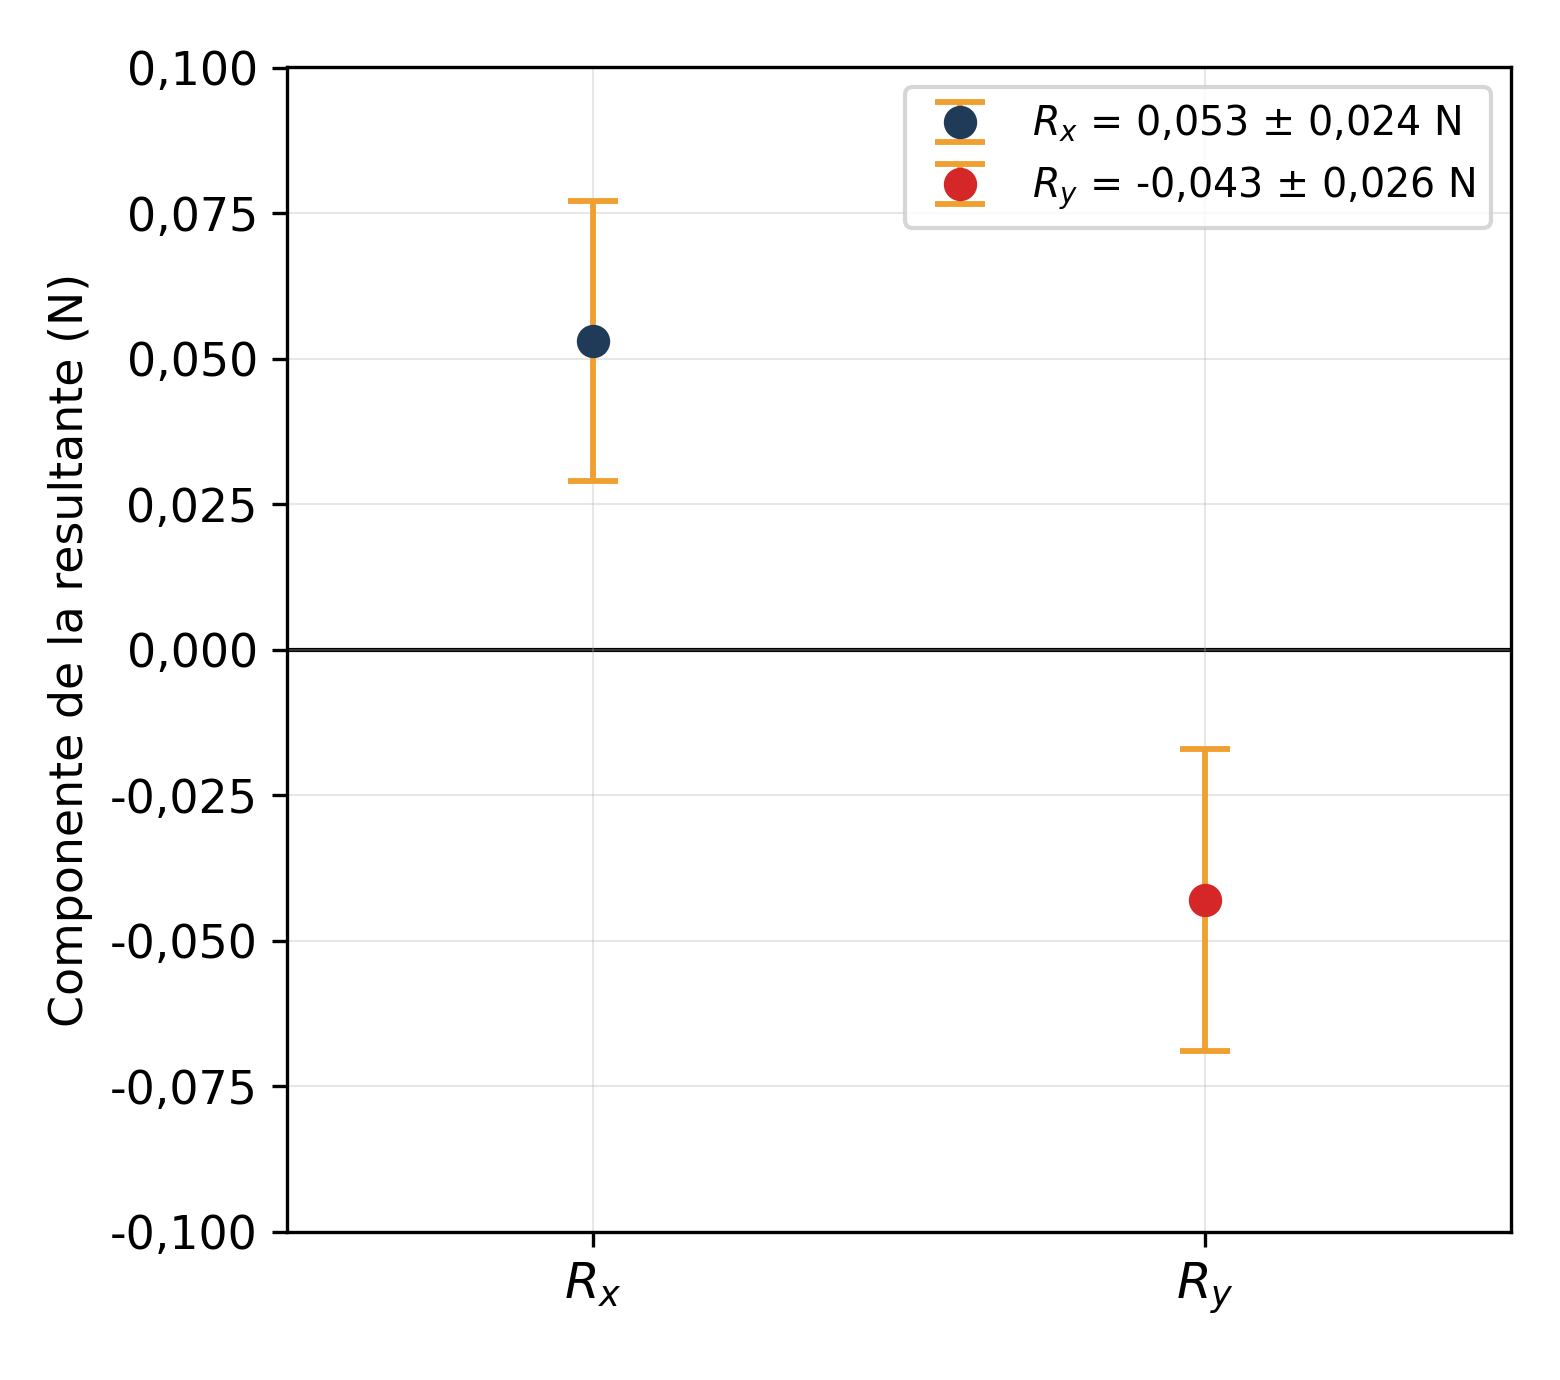
\includegraphics[width=0.4\textwidth]{grafico-error-config1.png}
    \caption{Gráficos de las componentes de la fuerza resultante $R_x$ y $R_y$ con barras de error en relación a la referencia teórica $y=0\,\mathrm{N}$ para la Configuración 1.}
    \label{fig:grafico-error-1}
\end{figure}

En la Fig. \ref{fig:grafico-error-1} se observa que ambas componentes de la resultante experimental se apartan de la referencia teórica: $R_x$ queda por encima de $y = 0\,\mathrm{N}$ y $R_y$ por debajo. En ninguno de los dos casos la barra de error cruza la línea de referencia: el intervalo de $R_x$ abarca de $0{,}029$ a $0{,}077\,\mathrm{N}$ y el de $R_y$ de $-0{,}069$ a $-0{,}017\,\mathrm{N}$. Por lo tanto, dentro de la incertidumbre estimada, el resultado experimental no es compatible con la condición de equilibrio traslacional $\sum \vec{F} = \vec{0}$; solo al ampliar el intervalo a $2\,\Delta R$ la componente $R_y$ pasa a ser compatible con cero, mientras que $R_x$ sigue quedando fuera por un margen pequeño. La discrepancia, de magnitud $|\vec{R}| \approx 0{,}07\,\mathrm{N}$, sugiere la presencia de fuentes de error sistemático no incluidas en la propagación: fricción en la polea que transmite $\vec{F}_1$ (lo que hace que la tensión efectiva sobre el anillo sea menor que $mg$), fricción entre el anillo central y el pivote de la mesa, y posibles desviaciones de cero o de calibración en los dinamómetros. El signo de $R_x > 0$ es coherente con esta interpretación, ya que indica que los dinamómetros registraron fuerzas menores a las necesarias para equilibrar el valor nominal de $\vec{F}_1$.
%Describan y analicen el gráfico obtenido. Indiquen si las barras de error de las componentes $R_x$ y $R_y$ cruzan la línea de referencia $y = 0\,\mathrm{N}$ y qué concluyen a partir de dicho cruce sobre la compatibilidad experimental con la condición de equilibrio traslacional.

\newpage


\subsection{Suma gráfica de los vectores de la Configuración 2}

\section{Configuración de Equilibrio 2}

En la segunda configuración se incrementó la masa suspendida a $m_2$, obteniéndose un peso $\vec{F}_1 = (0{,}995 \pm 0{,}001)\,\mathrm{N}$ posicionado a $0{,}00^\circ$. Las fuerzas $\vec{F}_2$ y $\vec{F}_3$ se registraron mediante dinamómetros a ángulos de $150{,}0^\circ$ y $210{,}0^\circ$ respectivamente. La incertidumbre angular fue de $\delta\theta = 2{,}50^\circ$ y la de los dinamómetros de $\delta F = 0{,}01\,\mathrm{N}$.

\begin{table}[h!]
\centering
\begin{tabular}{|c|c|c|}
\hline
\textbf{Fuerza} & \textbf{Módulo ($F \pm \delta F$)} & \textbf{Ángulo ($\theta \pm \delta \theta$)} \\ \hline
$F_1$ & $(0{,}995 \pm 0{,}001)\,\mathrm{N}$ & $(0{,}00 \pm 2{,}50)^\circ$ \\ \hline
$F_2$ & $(0{,}550 \pm 0{,}010)\,\mathrm{N}$ & $(150{,}00 \pm 2{,}50)^\circ$ \\ \hline
$F_3$ & $(0{,}560 \pm 0{,}010)\,\mathrm{N}$ & $(210{,}00 \pm 2{,}50)^\circ$ \\ \hline
\end{tabular}
\caption{Medición directa e indirecta de módulos y ángulos para la Configuración 2.}
\label{tab:config2-mediciones}
\end{table}

Los datos recolectados de esta configuración fueron registrados en la Tabla \ref{tab:config2-mediciones}. La representación gráfica de los vectores de esta configuración se puede ver en la Fig. \ref{fig:config2-vectores}.

\begin{figure}[h!]
    \centering
    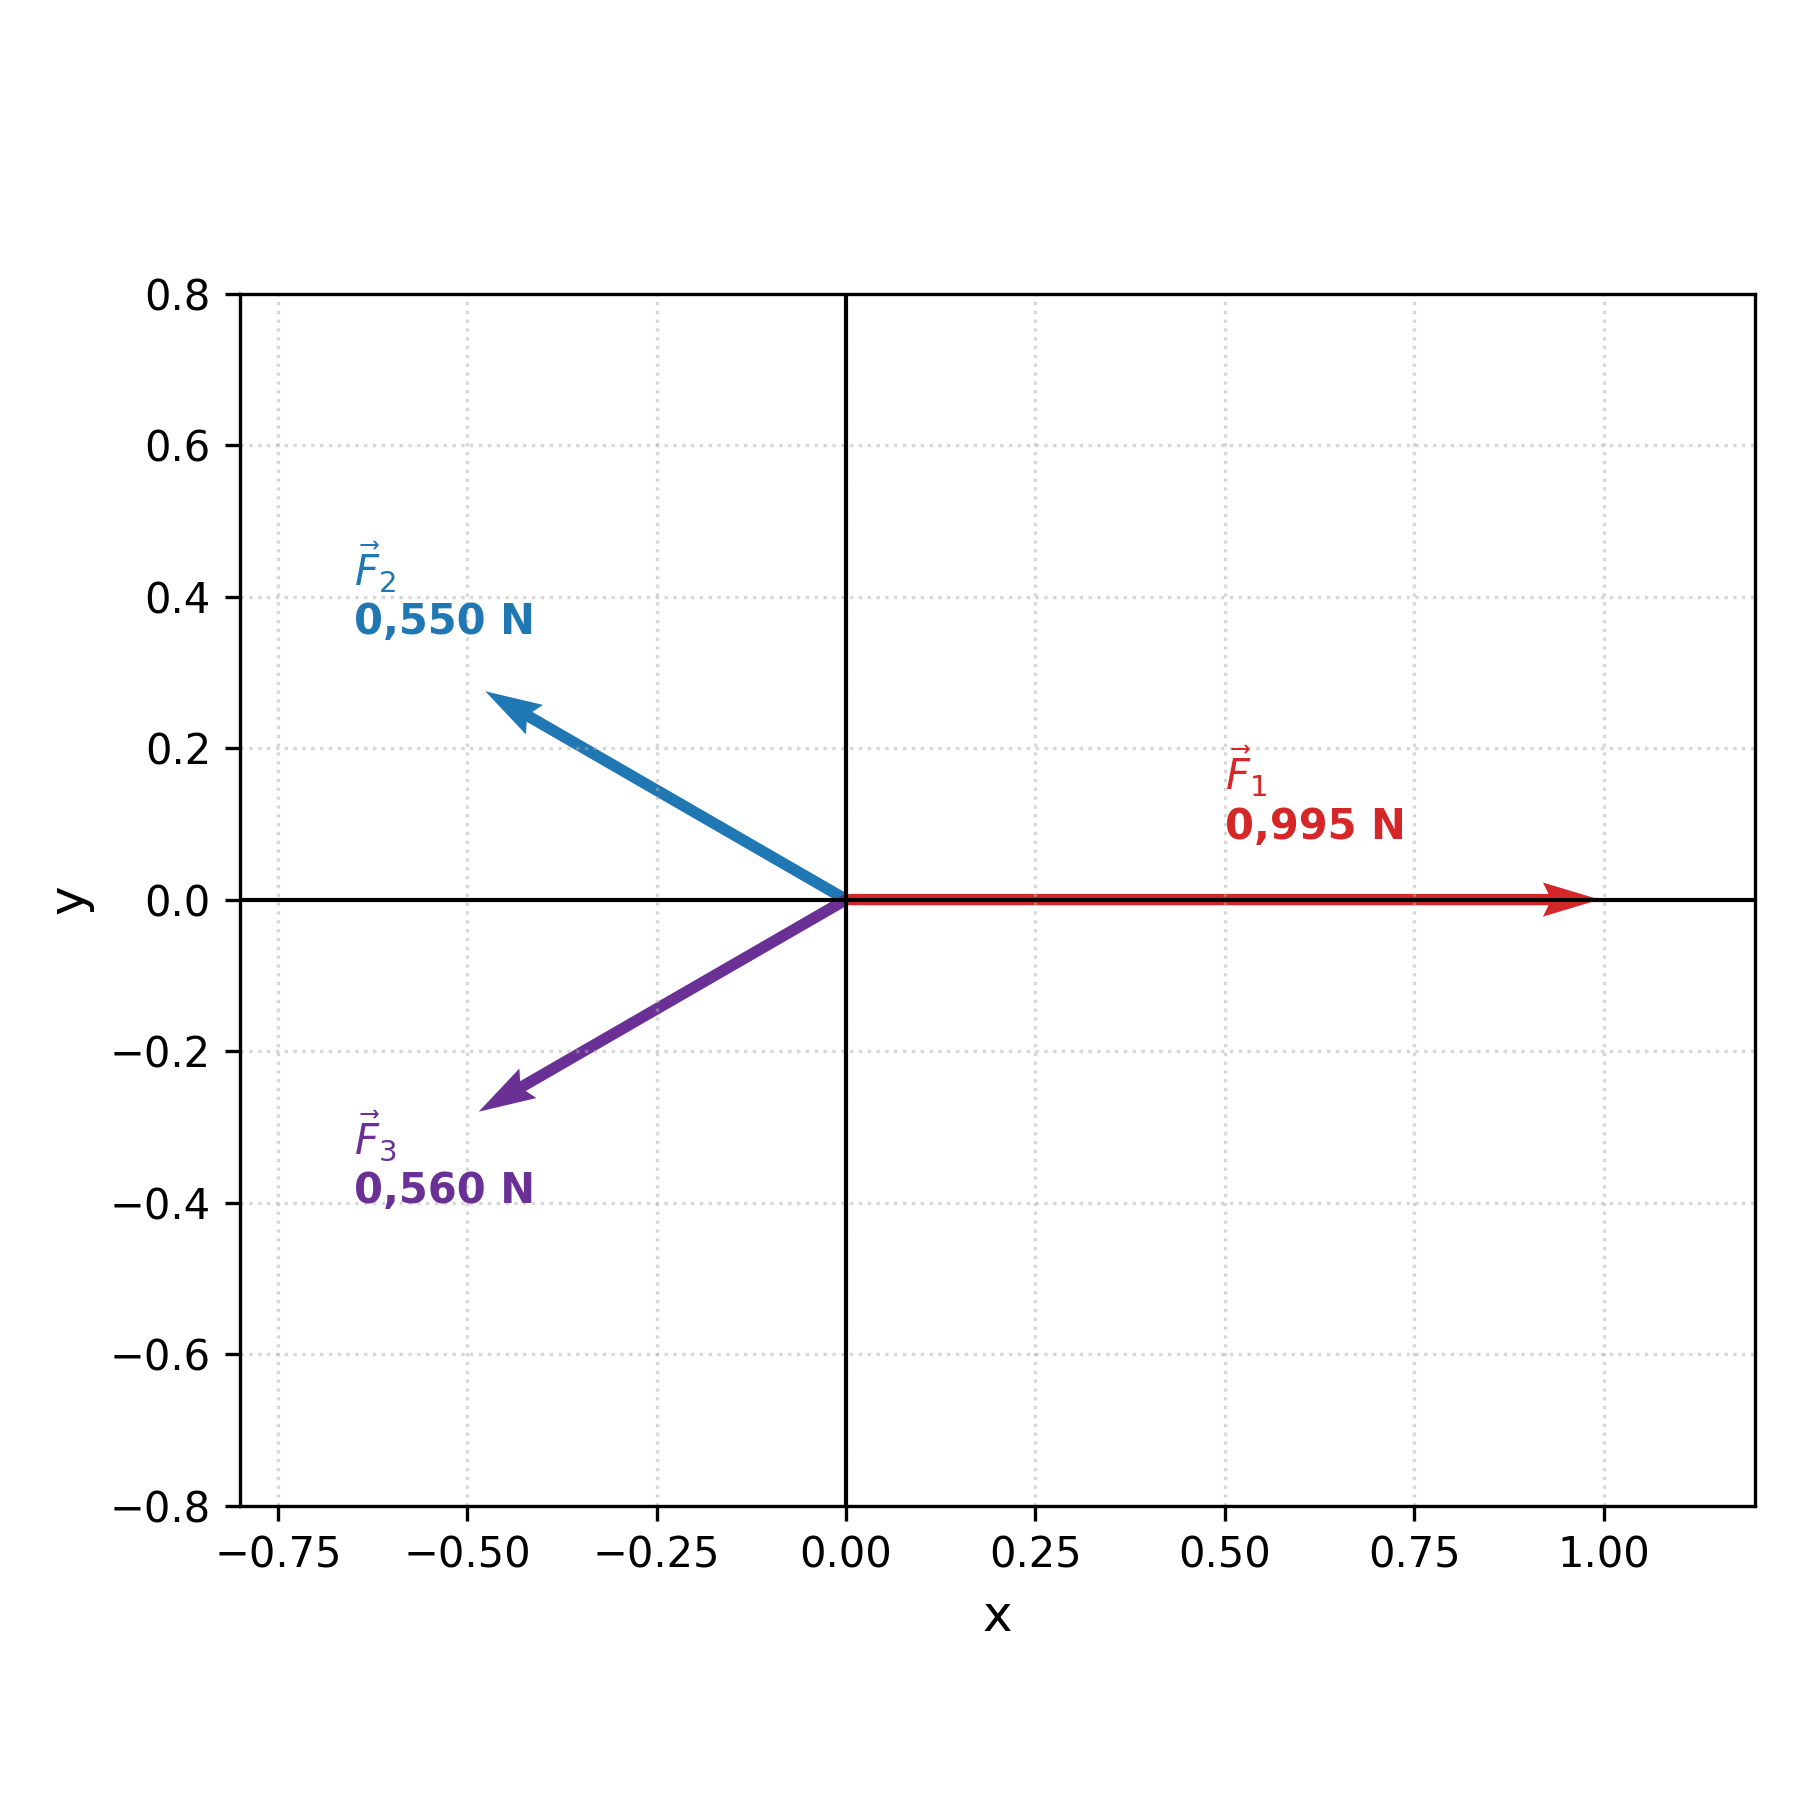
\includegraphics[width=0.4\textwidth]{config2-vectores.png}
    \caption{Representación en el sistema de referencia de los vectores $\vec{F}_1$, $\vec{F}_2$ y $\vec{F}_3$ (Configuración 2).}
    \label{fig:config2-vectores}
\end{figure}

\subsection{Suma gráfica de los vectores de la Configuración 2}

La suma gráfica de los vectores se puede ver en la Fig. \ref{fig:config2-poligono}.

\begin{figure}[h!]
    \centering
    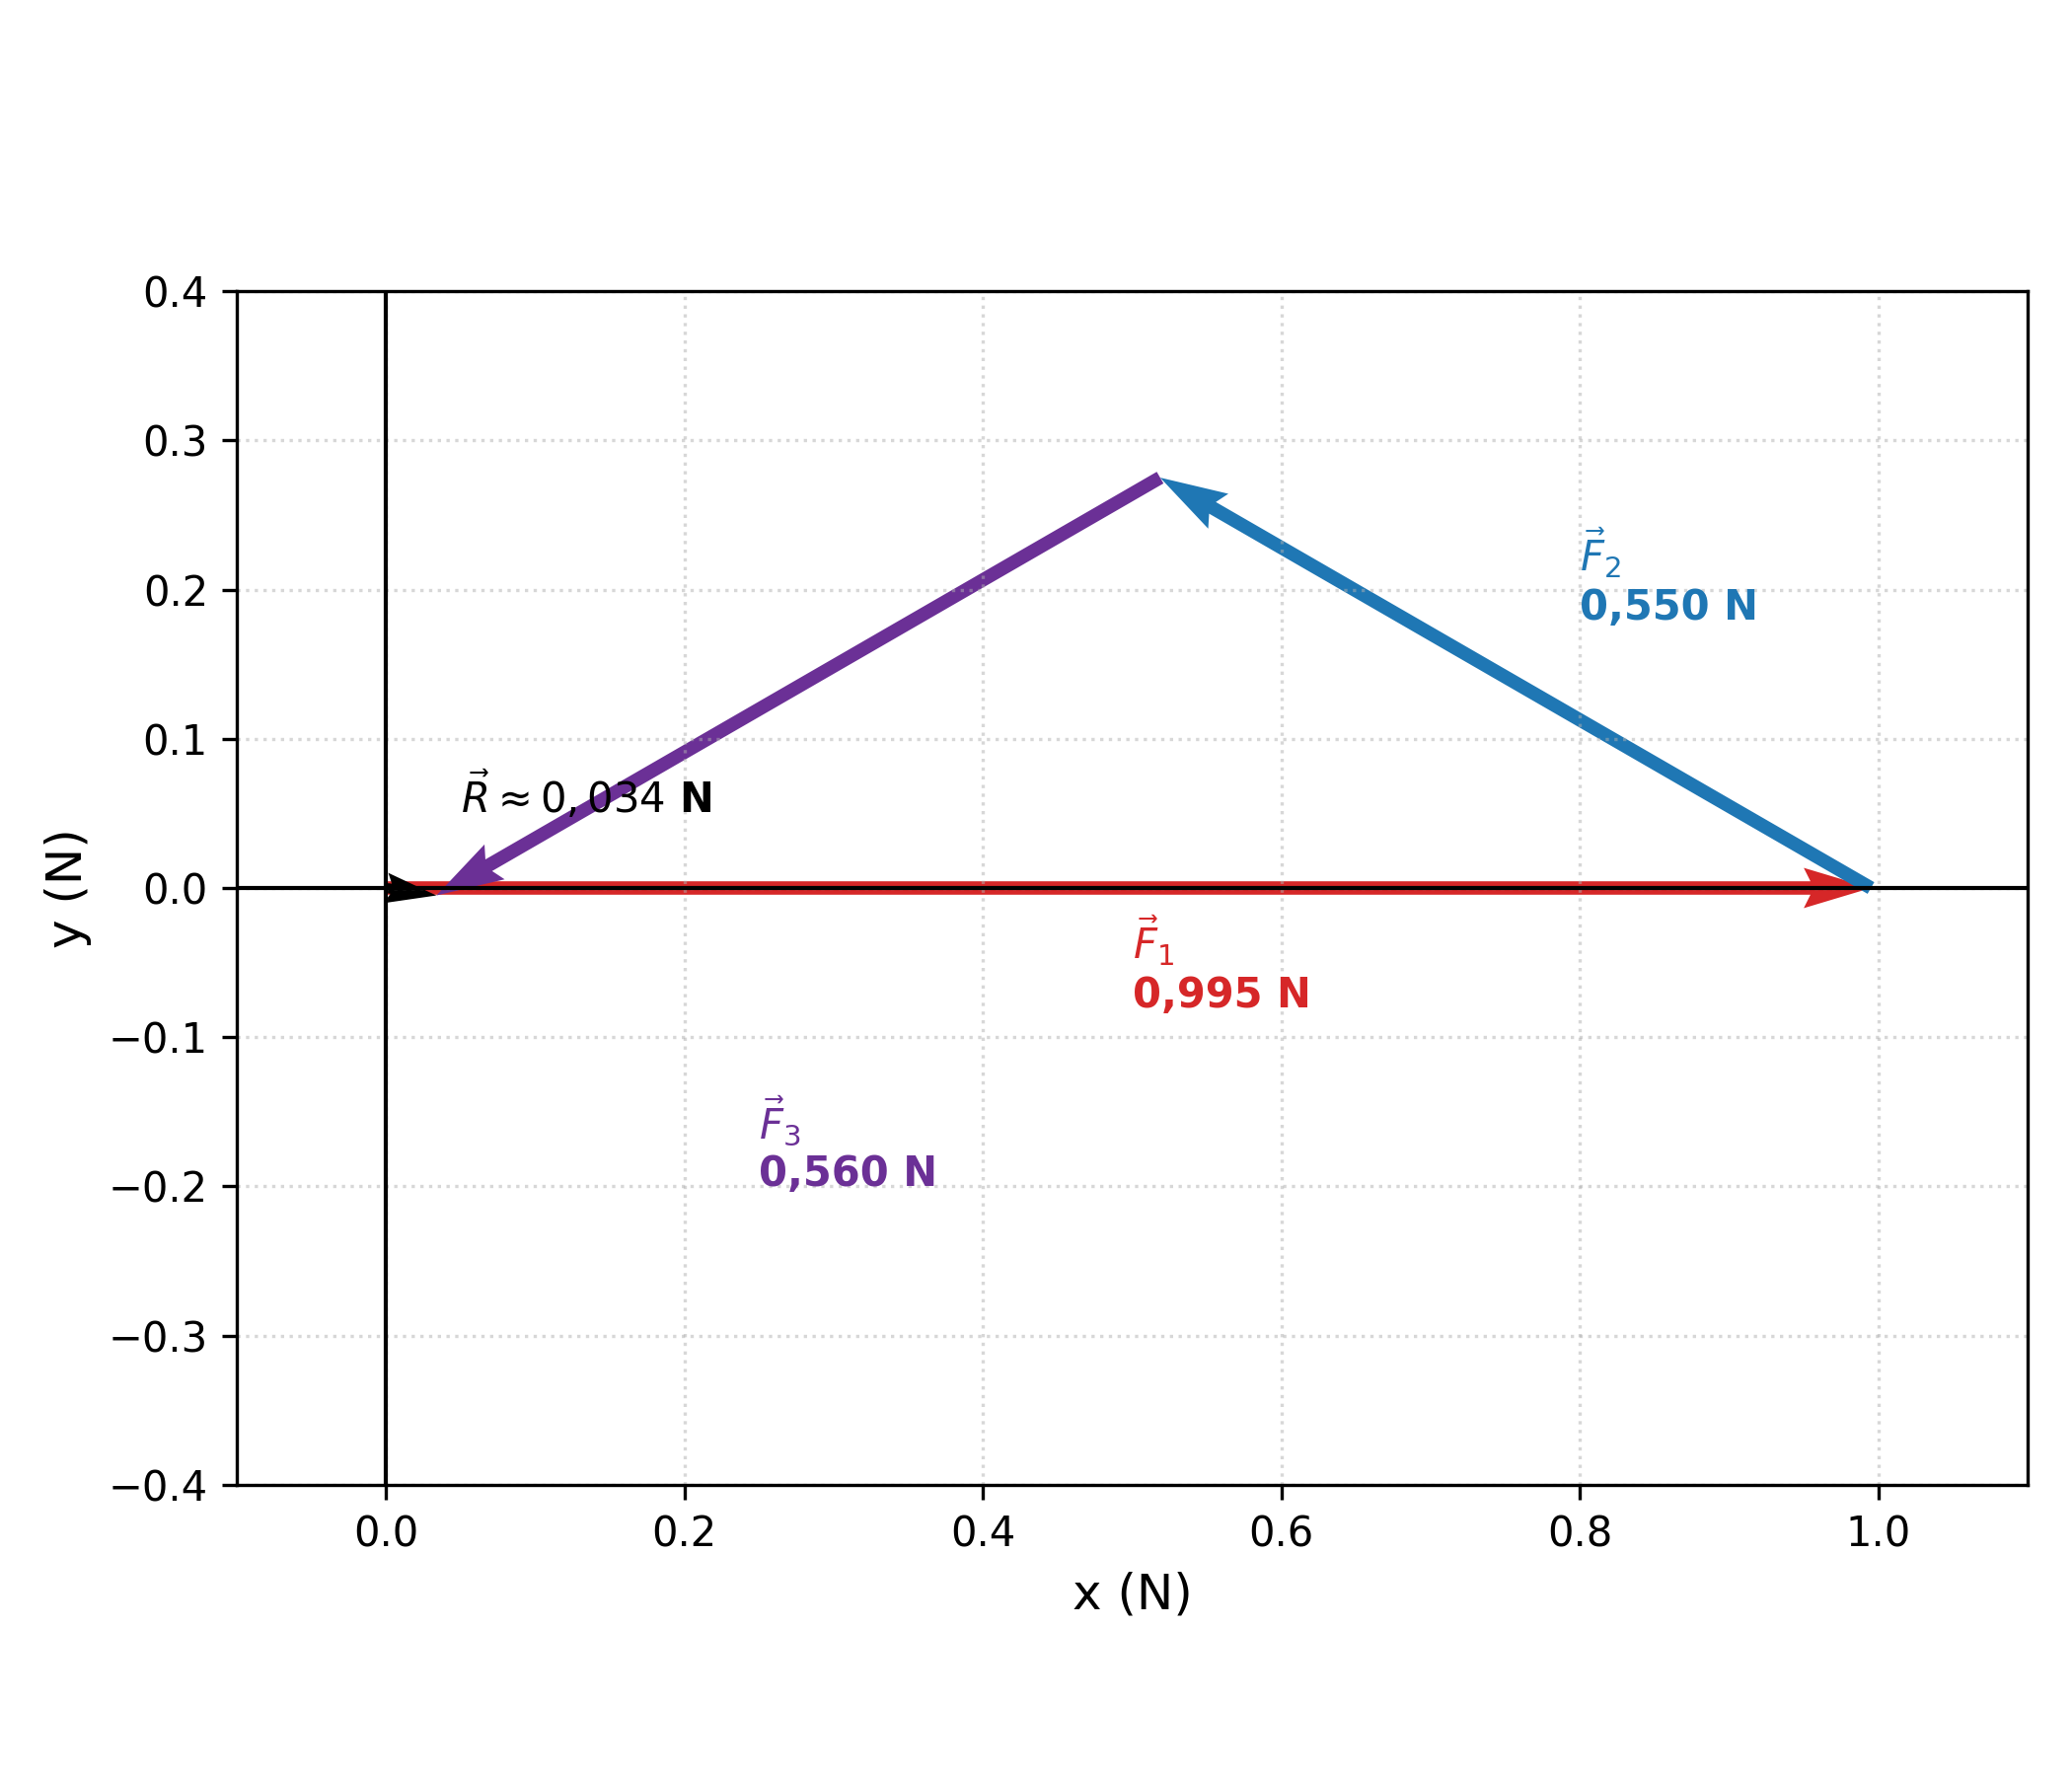
\includegraphics[width=0.4\textwidth]{config2-poligono.png}
    \caption{Suma gráfica mediante el método del polígono para la Configuración 2.}
    \label{fig:config2-poligono}
\end{figure}

Al construir el polígono vectorial a escala, se observa un leve desfase entre el origen del primer vector y el extremo del último, alcanzando una fuerza no equilibrada visible en el gráfico.

\subsection{Suma analítica}

Los vectores de la Configuración 2 separados en sus componentes están registrados en la Tabla \ref{tab:config2-componentes}.

\begin{table}[h!]
\centering
\begin{tabular}{|c|c|c|}
\hline
\textbf{Fuerza} & $F_x \pm \Delta F_x\,\mathrm{(N)}$ & $F_y \pm \Delta F_y\,\mathrm{(N)}$ \\ \hline
$F_1$ & $0{,}995 \pm 0{,}001$ & $0{,}000 \pm 0{,}043$ \\ \hline
$F_2$ & $-0{,}476 \pm 0{,}022$ & $0{,}275 \pm 0{,}021$ \\ \hline
$F_3$ & $-0{,}485 \pm 0{,}022$ & $-0{,}280 \pm 0{,}021$ \\ \hline
\end{tabular}
\caption{Componentes cartesianas e incertidumbres absolutas para la Configuración 2.}
\label{tab:config2-componentes}
\end{table}

Sumando estas componentes, el vector resultante es:

\begin{equation*}
\vec{R}_{\mathrm{exp, 2}} = (R_x \pm \Delta R_x)\,\uveci + (R_y \pm \Delta R_y)\,\uvecj = (0{,}034 \pm 0{,}031)\,\uveci + (-0{,}005 \pm 0{,}052)\,\uvecj\,\mathrm{N}
\end{equation*}

\subsection{Comparación de los resultados}

La Fig. \ref{fig:grafico-error-2} muestra la comparación gráfica entre la predicción teórica y el resultado experimental.

\begin{figure}[h!]
    \centering
    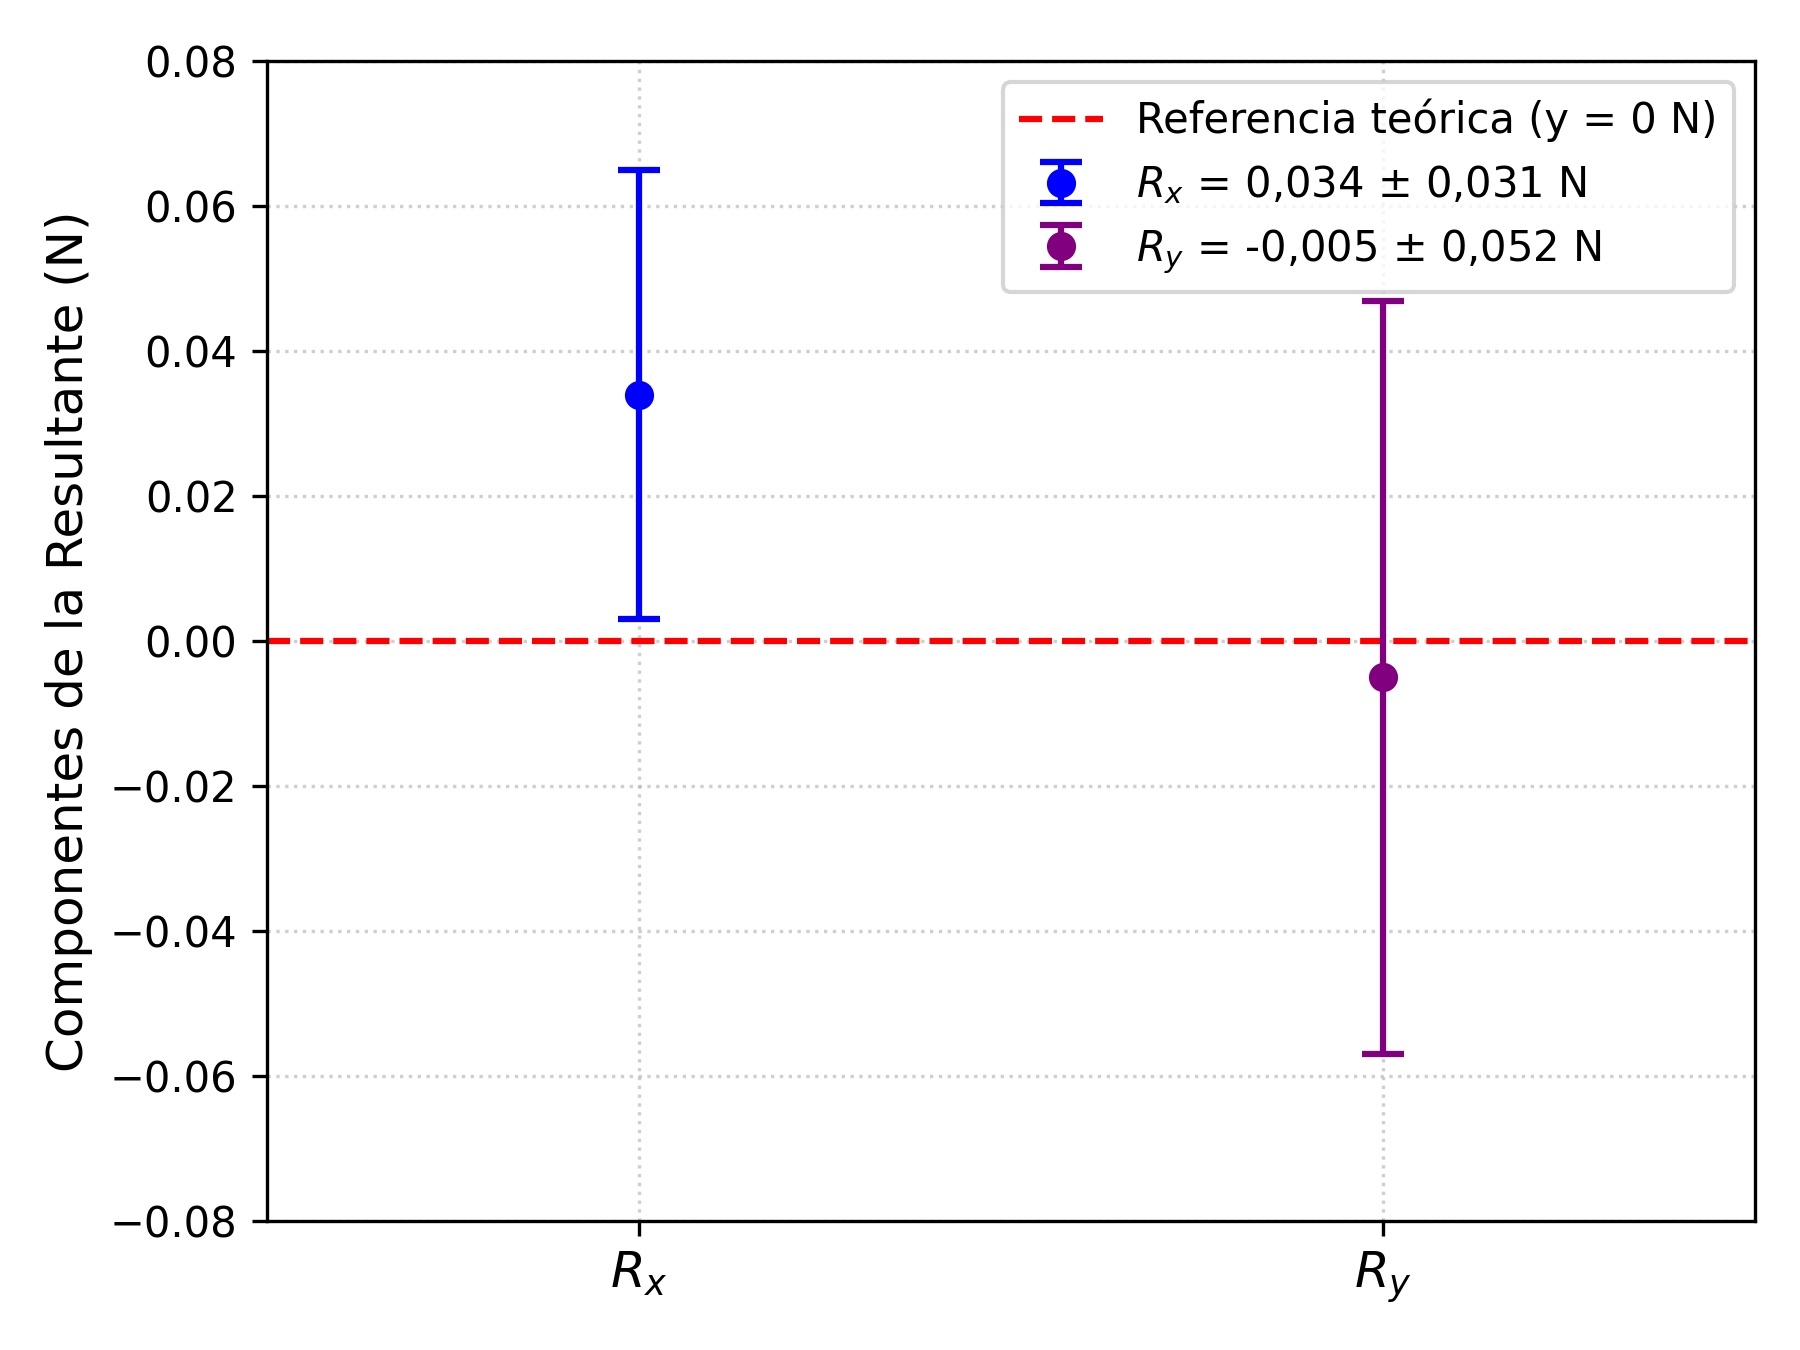
\includegraphics[width=0.4\textwidth]{grafico-error-config2.png}
    \caption{Gráficos de las componentes de la fuerza resultante $R_x$ y $R_y$ con barras de error en relación a la referencia teórica $y=0\,\mathrm{N}$ para la Configuración 2.}
    \label{fig:grafico-error-2}
\end{figure}

En la Fig. \ref{fig:grafico-error-2} se analiza el comportamiento de las componentes del vector resultante. La componente $R_y = (-0{,}005 \pm 0{,}052)\,\mathrm{N}$ cruza claramente la línea de referencia $y = 0\,\mathrm{N}$, por lo que es estadísticamente compatible con el equilibrio traslacional en el eje vertical. Para la componente $R_x = (0{,}034 \pm 0{,}031)\,\mathrm{N}$, la barra de error abarca desde $0{,}003\,\mathrm{N}$ hasta $0{,}065\,\mathrm{N}$, rozando la línea de referencia; con un intervalo de $2\Delta R_x$, esta componente también cruza $y = 0\,\mathrm{N}$. Por lo tanto, el sistema se aproxima satisfactoriamente a la condición de equilibrio, siendo las desviaciones menores atribuibles al roce mecánico en la polea y la sensibilidad de los dinamómetros.

\newpage
\section{Configuración de Equilibrio 3}

En la tercera configuración se utilizó tres masas suspendidas en la pole con dirección del eje $+x$. El peso de la masa, constituye la fuerza $\vec{F}_1$ ($\theta_1 = 0^\circ$). Las fuerzas $\vec{F}_2$ y $\vec{F}_3$ se aplicaron mediante dos dinamómetros fijados a $135^\circ$ y $300^\circ$ respecto al eje $+x$ (medidos en sentido antihorario). A diferencia de la Configuración 1, en este caso las fuerzas no están separadas simétricamente, y los módulos de $\vec{F}_2$ y $\vec{F}_3$ son considerablemente mayores que el de $\vec{F}_1$. La incertidumbre angular de la mesa se estimó en $\delta\theta = 2{,}5^\circ$ y la de los dinamómetros en $\delta F = 0{,}01\,\mathrm{N}$.
%Describan la tercera configuración de equilibrio utilizada, considerando la cantidad de masas suspendidas, la disposición de los dinamómetros y los ángulos seleccionados.

\begin{table}[h!]
\centering
\begin{tabular}{|c|c|c|}
\hline
\textbf{Fuerza} & \textbf{Módulo ($F \pm \delta F$)} & \textbf{Ángulo ($\theta \pm \delta \theta$)} \\ \hline
$F_1$ & $(1{,}495 \pm 0{,}010)\mathrm{N}$ & $(0{,}0 \pm 2{,}50)^\circ$  \\ \hline
$F_2$ & $(4{,}59 \pm 0{,}01)\mathrm{N}$ & $(135{,}0 \pm 2{,}50)^\circ$  \\ \hline
$F_3$ & $(3{,}69 \pm 0{,}01)\mathrm{N}$ & $(300{,}0 \pm 2{,}50)^\circ$  \\ \hline
\end{tabular}
\caption{Medición directa e indirecta de módulos y ángulos para la Configuración 3.}
\label{tab:config3-mediciones}
\end{table}

Los datos recolectados de esta configuración fueron registrados en la Tabla \ref{tab:config3-mediciones}. El módulo de $\vec{F}_1$ corresponde al peso de la masa, calculado como $F_1 = mg$. Para obtener $\delta F_1$, se realizó propagación de error.
\begin{equation*}
F_1 = mg = ({0{,}1524}\,\mathrm{kg})(9{,}81\,\mathrm{m/s^2}) = 1{,}495\,\mathrm{N}
\end{equation*}
\begin{equation*}
\delta F_1 = \sqrt{(9{,}81 \times 0{,}00001)^2 + (0{,}1524 \times 0{,}01)^2}\;\mathrm{N} \approx 0{,}01\,\mathrm{N} = \sqrt{(9{,}81 \times 0{,}00001)^2 + (0{,}1524 \times 0{,}01)^2}\;\mathrm{N} \approx 0{,}01\,\mathrm{N}
\end{equation*}

La representación gráfica de los vectores de esta configuración se puede ver en la Fig. \ref{fig:config3-vectores}.

\begin{figure}[h!]
    \centering
    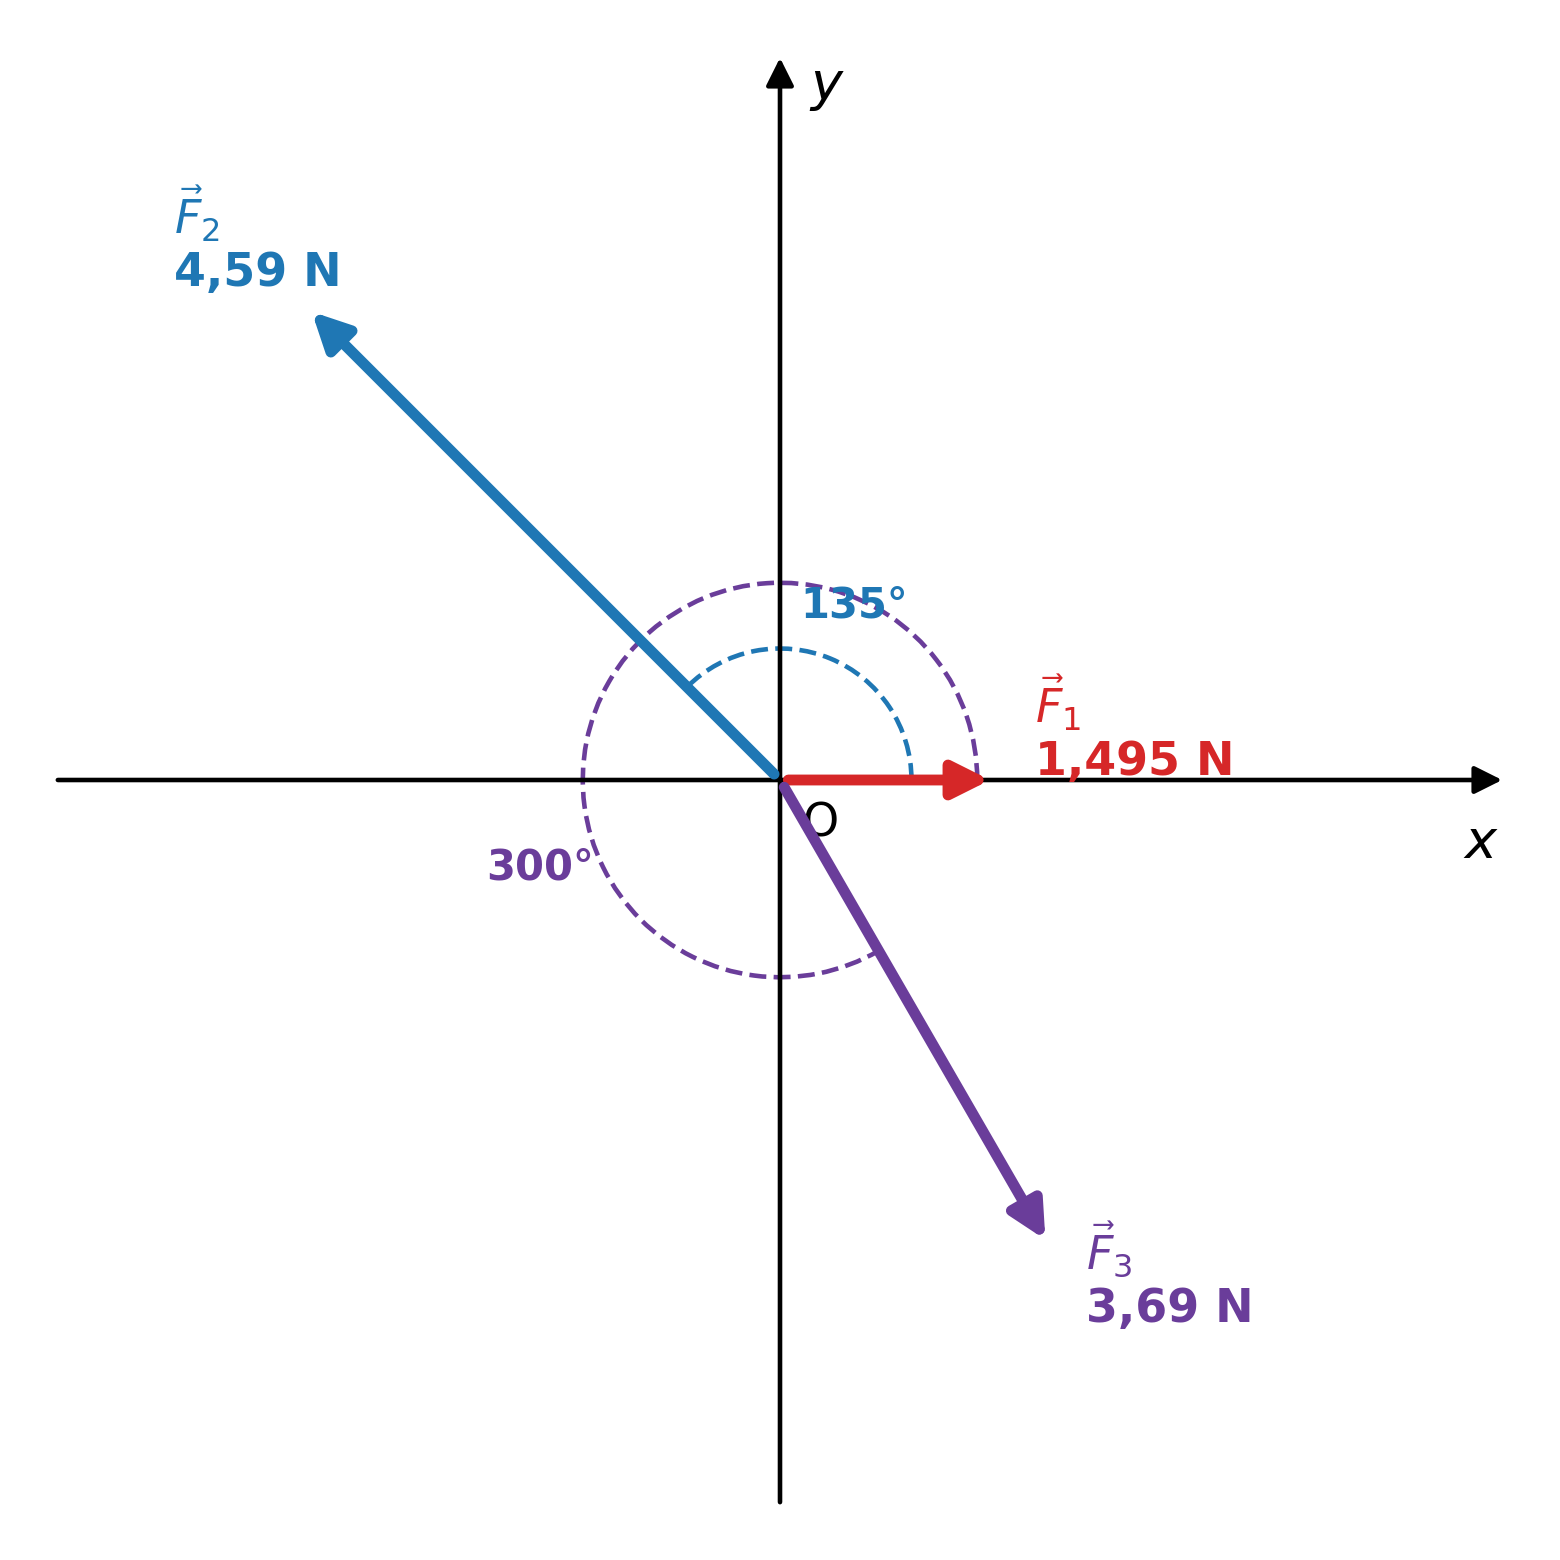
\includegraphics[width=0.4\textwidth]{config3-vectores.png}
    \caption{Representación en el sistema de referencia de los vectores $\vec{F}_1$, $\vec{F}_2$ y $\vec{F}_3$ (Configuración 3).}
    \label{fig:config3-vectores}
\end{figure}

\subsection{Suma gráfica de los vectores de la Configuración 3}

La suma gráfica de los vectores se puede ver en la Fig. \ref{fig:config3-poligono}.

\begin{figure}[h!]
    \centering
    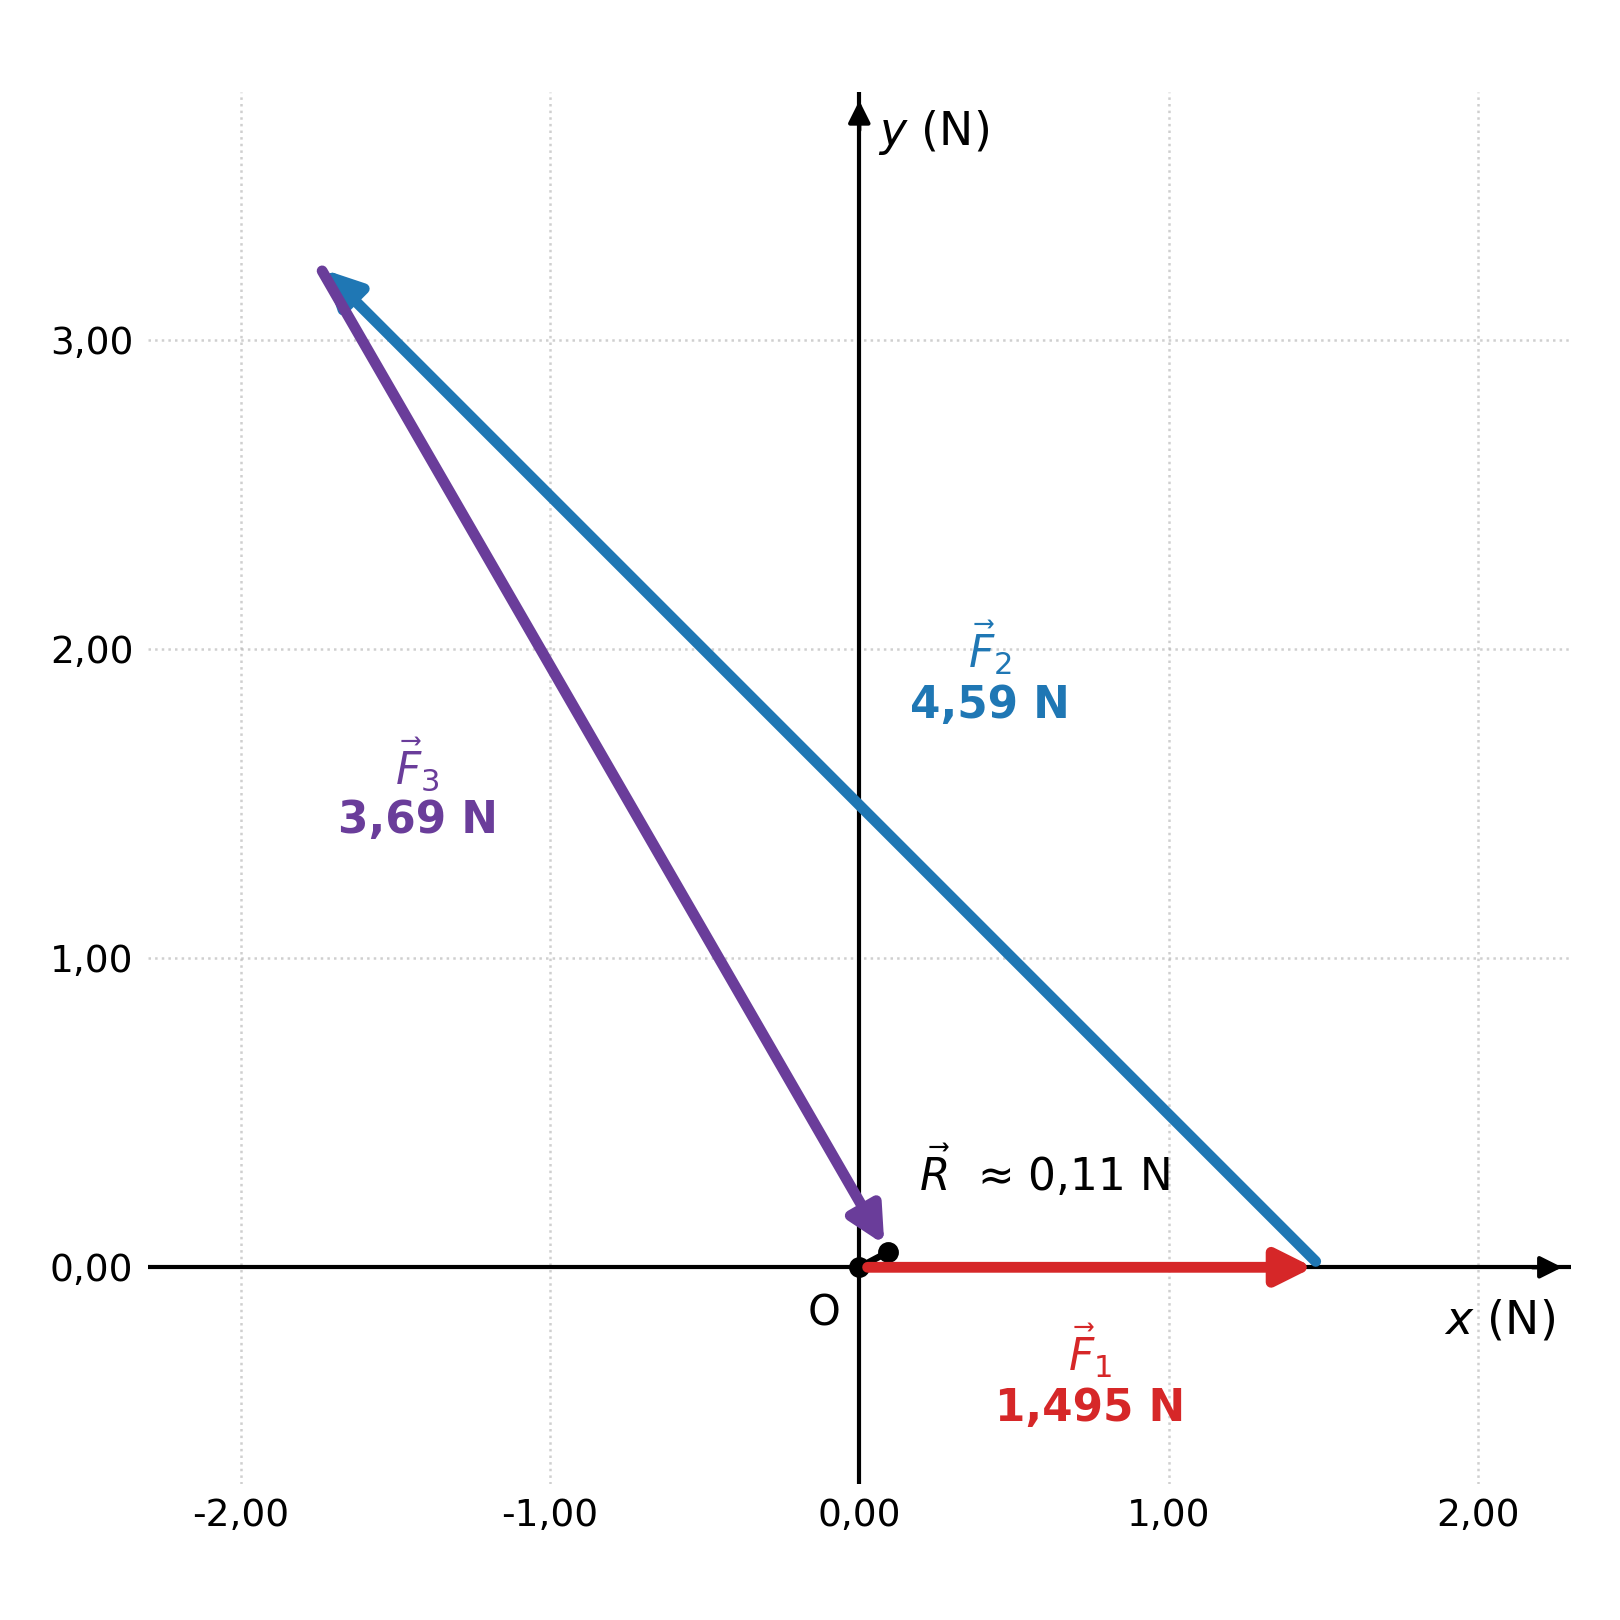
\includegraphics[width=0.4\textwidth]{config3-poligono.png}
    \caption{Suma gráfica mediante el método del polígono para la Configuración 3.}
    \label{fig:config3-poligono}
\end{figure}

Al trazar los vectores, el polígono se cierra casi por completo: el extremo de $\vec{F}_3$ queda muy próximo al origen de $\vec{F}_1$, con una abertura aproximadamente de $0{,}11\,\mathrm{N}$. Ya que los módulos de las fuerzas, son del orden de varios newtons, esta discrepancia es pequeña (menor al $3\,\%$ del módulo de $\vec{F}_2$), por lo que gráficamente el sistema se muestra consistente con el equilibrio.
%Comenten cualitativamente si el polígono se cierra correctamente o si existe alguna discrepancia gráfica visible.

\subsection{Suma analítica de los vectores de la Configuración 3}

Los vectores de la Configuración 3 separados en sus componentes están registrados en la Tabla \ref{tab:config3-componentes}.

\begin{table}[h!]
\centering
\begin{tabular}{|c|c|c|}
\hline
\textbf{Fuerza} & $F_x \pm \Delta F_x\mathrm{(N)}$ & $F_y \pm \Delta F_y\mathrm{(N)}$ \\ \hline
$F_1$ & $1{,}50 \pm 0{,}01$ & $0{,}00 \pm 0{,}07$  \\ \hline
$F_2$ & $-3{,}25 \pm 0{,}14$ & $3{,}25 \pm 0{,}14$  \\ \hline
$F_3$ & $1{,}85 \pm 0{,}14$ & $-3{,}20 \pm 0{,}08$  \\ \hline
\end{tabular}
\caption{Componentes cartesianas e incertidumbres absolutas para la Configuración 3.}
\label{tab:config3-componentes}
\end{table}

Sumando estas componentes, el vector resultante es:

\begin{equation*}
\vec{R}_{\mathrm{exp, 3}} = (R_x \pm \Delta R_x)\,\uveci + (R_y \pm \Delta R_y)\,\uvecj = (0{,}09 \pm 0{,}20)\,\uveci + (0{,}05 \pm 0{,}18)\,\uvecj\,\mathrm{N}
\end{equation*}

\subsection{Comparación de los resultados}

La Fig. \ref{fig:grafico-error-3} muestra la comparación gráfica entre la predicción teórica y el resultado experimental.

\begin{figure}[h!]
    \centering
    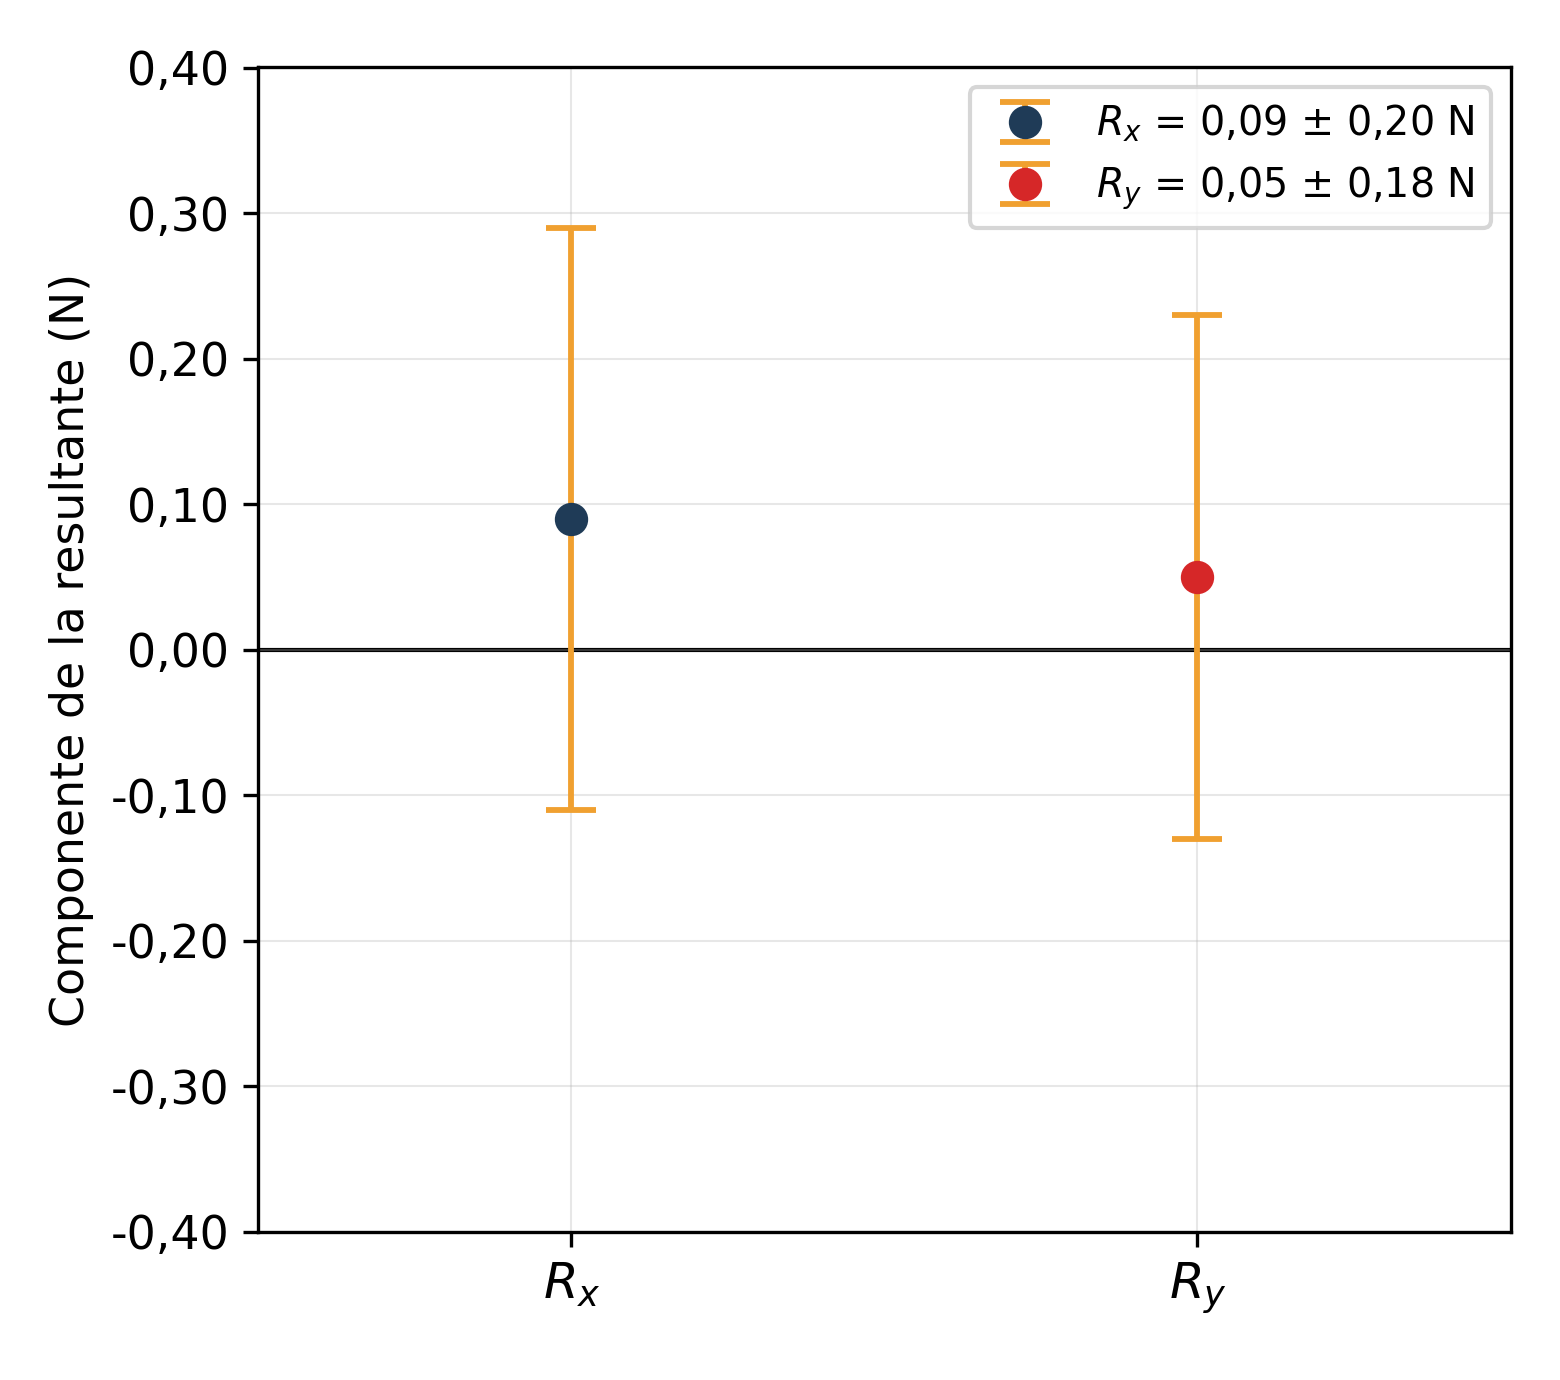
\includegraphics[width=0.4\textwidth]{grafico-error-config3.png}
    \caption{Gráficos de las componentes de la fuerza resultante $R_x$ y $R_y$ con barras de error en relación a la referencia teórica $y=0\,\mathrm{N}$ para la Configuración 3.}
    \label{fig:grafico-error-3}
\end{figure}

En la Fig. \ref{fig:grafico-error-3} se observa que ambas componentes de la resultante experimental toman valores positivos pequeños, $R_x = 0{,}09\,\mathrm{N}$ y $R_y = 0{,}05\,\mathrm{N}$. En ambos casos la barra de error cruza la línea de referencia $y = 0\,\mathrm{N}$: el intervalo de $R_x$ abarca de $-0{,}11$ a $0{,}29\,\mathrm{N}$ y el de $R_y$ de $-0{,}13$ a $0{,}23\,\mathrm{N}$. Cabe notar que las incertidumbres de esta configuración son mayores que en la Configuración 1, debido principalmente a que la incertidumbre angular ($\delta\theta = 2{,}5^\circ$) se multiplica por módulos de fuerza más grandes, lo que amplía las barras de error de las componentes de $\vec{F}_2$ y $\vec{F}_3$.
%Describan y analicen el gráfico obtenido. Indiquen si las barras de error de las componentes $R_x$ y $R_y$ cruzan la línea de referencia $y = 0\,\mathrm{N}$ y qué concluyen a partir de dicho cruce sobre la compatibilidad experimental con la condición de equilibrio traslacional.

\newpage
\section{Análisis y conclusiones}

Durante la experiencia de laboratorio se estudió la condición de equilibrio traslacional y la suma de fuerzas obtenidas mediante un sistema, el cual se llevó a cabo al borde de una mesa con una tabla graduada, en la cual ubicamos el eje $+x$ en dirección hacia la suspensión de masas. También ocupamos dinamómetros los cuales nos entregan la magnitud de la fuerza ejercida y los ángulos; todo esto fue registrado, construyendo además la representación gráfica de las fuerzas mediante el método del polígono (Sección \ref{Procedimiento-Parte-1}). Luego, se realizó un análisis del sistema, descomponiendo cada vector en sus componentes cartesianas y aplicando la propagación de incertidumbres absolutas a través de derivadas parciales para calcular la fuerza resultante experimental $\vec{R}_{\text{exp}}$ (Sección \ref{Procedimiento-Parte-2}). Finalmente, comparamos los resultados experimentales con el valor teórico esperado de $y = 0\,\mathrm{N}$ mediante gráficos de componentes con barras de error (Sección \ref{Procedimiento-Parte-3}).

Físicamente, la expresión $\sum \vec{F} = \vec{0}$ representa el cumplimiento de la primera condición de equilibrio, esto establece que para que una partícula se mantenga en reposo, la suma de todas las fuerzas aplicadas debe ser nula. Al comparar el método gráfico con el analítico, se evidencia que el análisis matemático nos da una precisión mucho mayor. El método del polígono es muy útil visualmente, pero depende del trazo a mano, la escala y la precisión con el transportador. En cambio, el método analítico considera directamente los errores de los instrumentos y calcula numéricamente la propagación del error, permitiendo saber si el resultado se acerca al cero teórico.

En la Configuración 1, se notaron diferencias entre la medición experimental y lo esperado teóricamente. Gráficamente, el polígono no llegó a cerrarse del todo, dejando una abertura visible de aproximadamente un $14\,\%$ respecto a la fuerza $\vec{F}_1$. Esto coincide con el cálculo analítico, donde obtuvimos una fuerza resultante no nula de $\vec{R}_{\text{exp, 1}} = (0{,}053 \pm 0{,}024)\,\uveci + (-0{,}043 \pm 0{,}026)\,\uvecj\,\mathrm{N}$. Al revisar el gráfico de barras de error, se observa que ninguna de las dos componentes cruza la línea $y = 0\,\mathrm{N}$ para $1\Delta R$, por lo que, dentro de ese margen de incerteza, el resultado no es estrictamente compatible con el equilibrio teórico.

En la Configuración 2, los resultados se acercaron bastante más a la predicción teórica. El cálculo analítico dio una resultante $\vec{R}_{\text{exp, 2}} = (0{,}034 \pm 0{,}031)\,\uveci + (-0{,}005 \pm 0{,}052)\,\uvecj\,\mathrm{N}$. En este caso, la barra de error de la componente $R_y$ cruza claramente la línea de referencia $y = 0\,\mathrm{N}$, resultando compatible con cero. Para la componente $R_x$, aunque con $1\Delta R_x$ queda ligeramente fuera ($0{,}003$ a $0{,}065\,\mathrm{N}$), basta con considerar un intervalo de $2\Delta R_x$ para que también pase a cruzar la línea cero. Esto demuestra la importancia de analizar las barras de error, porque una barra que cruza la línea $y = 0\,\mathrm{N}$ indica que el valor nulo está dentro del margen de incerteza experimental y que las diferencias observadas son solo variaciones normales del experimento.

En la Configuración 3 aumentamos las cargas y usamos tres masas con una disposición asimétrica, ubicando los dinamómetros a $135{,}0^\circ$ y $300{,}0^\circ$. Al armarla, el polígono gráfico se cerró harto mejor que en la primera prueba, dejando una abertura pequeña de cerca de $0{,}11\,\mathrm{N}$ (menos del $3\,\%$ de $\vec{F}_2$). Analíticamente obtuvimos una resultante de $\vec{R}_{\mathrm{exp, 3}} = (0{,}09 \pm 0{,}20)\,\uveci + (0{,}05 \pm 0{,}18)\,\uvecj\,\mathrm{N}$. Al revisar el gráfico de errores, las barras de ambas componentes cruzaron sin problemas la línea de referencia $y = 0\,\mathrm{N}$ (con intervalos que van desde $-0{,}11$ hasta $0{,}29\,\mathrm{N}$ para $x$, y de $-0{,}13$ hasta $0{,}23\,\mathrm{N}$ para $y$). Aquí las barras se vieron más anchas que en las configuraciones anteriores porque la incertidumbre angular de $2{,}5^\circ$ se multiplica por módulos de fuerza bastante más grandes, ensanchando de forma lógica el margen de error instrumental.

A pesar de que las tres configuraciones compartían la característica de estar centradas y estables en la mesa de trabajo, fue normal obtener resultantes analíticas ligeramente distintas de cero. Esto se explica porque el ojo humano percibe equilibrio dentro de una "zona de reposo" provocada por las imperfecciones del montaje. Específicamente, se identificaron tres fuentes principales de error experimental:
\begin{enumerate}[leftmargin=*]
\item \textbf{Roce en las poleas:} La fricción en el eje de las poleas disminuye la tensión de las cuerdas, haciendo que la fuerza ejercida sobre el anillo central sea menor al peso $mg$ de las masas colgadas.
\item \textbf{Fricción en el pivote del anillo central:} La fricción del anillo con la guía vertical permite que se mantenga quieto aunque exista una pequeña fuerza no equilibrada actuando sobre él.
\item \textbf{Incertidumbre de lectura y alineación:} La resolución de la mesa de fuerzas ($\delta\theta = 2{,}5^\circ$) y las pequeñas desviaciones de cero en los dinamómetros analógicos ($\delta F = 0{,}01\,\mathrm{N}$) generan variaciones al descomponer los vectores.
\end{enumerate}

En conclusión, se pudo verificar experimentalmente el comportamiento de la suma vectorial de fuerzas y la validez de la primera condición de equilibrio en el plano. Comprobamos que el cálculo analítico por componentes junto con la propagación de errores es fundamental para evaluar un experimento real, ya que nos permite diferenciar entre errores asociados a los instrumentos y las variaciones de las mediciones de laboratorio.

\textbf{\underline{Extensión máxima del informe:} indefinida}.

\begin{thebibliography}{99}

\bibitem{libro} Nombre del autor. \textit{Título del libro}. Año.

\bibitem{apunte} Nombre del profesor. \textit{Nombre del curso}. Semestre y año en el que fue entregado el apunte.

\bibitem{web} TikTok de @usuario. Disponible en: \url{https://www.tiktok.com/}.

\end{thebibliography}

\end{document}
